%!TEX TS-program = xelatex
\documentclass[notes,12pt, aspectratio=169]{beamer}

\usepackage{amsmath,amsfonts,amssymb,amsthm,mathtools}  % пакеты для математики
\usepackage{minted}

\usepackage[english, russian]{babel} % выбор языка для документа
\usepackage[utf8]{inputenc} % задание utf8 кодировки исходного tex файла
\usepackage[X2,T2A]{fontenc}        % кодировка

\usepackage{fontspec}         % пакет для подгрузки шрифтов
\setmainfont{Helvetica}  % задаёт основной шрифт документа

% why do we need \newfontfamily:
% http://tex.stackexchange.com/questions/91507/
\newfontfamily{\cyrillicfonttt}{Helvetica}
\newfontfamily{\cyrillicfont}{Helvetica}
\newfontfamily{\cyrillicfontsf}{Helvetica}

\usepackage{unicode-math}     % пакет для установки математического шрифта
% \setmathfont{Neo Euler} % шрифт для математики

\usepackage{polyglossia}      % Пакет, который позволяет подгружать русские буквы
\setdefaultlanguage{russian}  % Основной язык документа
\setotherlanguage{english}    % Второстепенный язык документа

% Шрифт для кода
\setmonofont[Scale=0.85]{Monaco}
\usepackage{verbments}

\usepackage{pgfpages}
% These slides also contain speaker notes. You can print just the slides,
% just the notes, or both, depending on the setting below. Comment out the want
% you want.
%\setbeameroption{hide notes} % Only slide
%\setbeameroption{show only notes} % Only notes
%\setbeameroption{show notes on second screen=right} % Both

\usepackage{array}

\usepackage{tikz}
\usepackage{verbatim}
\setbeamertemplate{note page}{\pagecolor{yellow!5}\insertnote}
\usetikzlibrary{positioning}
\usetikzlibrary{snakes}
\usetikzlibrary{calc}
\usetikzlibrary{arrows}
\usetikzlibrary{decorations.markings}
\usetikzlibrary{shapes.misc}
\usetikzlibrary{matrix,shapes,arrows,fit,tikzmark}

\usepackage{hyperref}
\usepackage{lipsum}
\usepackage{multimedia}
\usepackage{multirow}
\usepackage{dcolumn}
\usepackage{bbm}
\newcolumntype{d}[0]{D{.}{.}{5}}

\usepackage{changepage}
\usepackage{appendixnumberbeamer}
\newcommand{\beginbackup}{
   \newcounter{framenumbervorappendix}
   \setcounter{framenumbervorappendix}{\value{framenumber}}
   \setbeamertemplate{footline}
   {
     \leavevmode%
     \hline
     box{%
       \begin{beamercolorbox}[wd=\paperwidth,ht=2.25ex,dp=1ex,right]{footlinecolor}%
%         \insertframenumber  \hspace*{2ex} 
       \end{beamercolorbox}}%
     \vskip0pt%
   }
 }
\newcommand{\backupend}{
   \addtocounter{framenumbervorappendix}{-\value{framenumber}}
   \addtocounter{framenumber}{\value{framenumbervorappendix}} 
}

% для имитации питоновского синтаксиса 
\newcommand{\pgr}[1]{{\color{green} \textbf{#1}}}


%%%%%%%%%% Работа с картинками %%%%%%%%%
\usepackage{graphicx}                  % Для вставки рисунков
\usepackage{graphics}
\graphicspath{{images/},{imagess/}}    % можно указать папки с картинками
\usepackage{wrapfig}                   % Обтекание рисунков и таблиц текстом

\usepackage[space]{grffile}
\usepackage{booktabs}

% These are my colors -- there are many like them, but these ones are mine.
\definecolor{blue}{RGB}{0,114,178}
\definecolor{red}{RGB}{213,94,0}
\definecolor{yellow}{RGB}{240,228,66}
\definecolor{green}{RGB}{0,128, 0}

\hypersetup{
  colorlinks=false,
  linkbordercolor = {white},
  linkcolor = {blue}
}


%% I use a beige off white for my background
\definecolor{MyBackground}{RGB}{255,253,218}

%% Uncomment this if you want to change the background color to something else
%\setbeamercolor{background canvas}{bg=MyBackground}

%% Change the bg color to adjust your transition slide background color!
\newenvironment{transitionframe}{
  \setbeamercolor{background canvas}{bg=yellow}
  \begin{frame}}{
    \end{frame}
}

\setbeamercolor{frametitle}{fg=blue}
\setbeamercolor{title}{fg=black}
\setbeamertemplate{footline}[frame number]
\setbeamertemplate{navigation symbols}{} 
\setbeamertemplate{itemize items}{-}
\setbeamercolor{itemize item}{fg=blue}
\setbeamercolor{itemize subitem}{fg=blue}
\setbeamercolor{enumerate item}{fg=blue}
\setbeamercolor{enumerate subitem}{fg=blue}
\setbeamercolor{button}{bg=MyBackground,fg=blue,}


% If you like road maps, rather than having clutter at the top, have a roadmap show up at the end of each section 
% (and after your introduction)
% Uncomment this is if you want the roadmap!
% \AtBeginSection[]
% {
%    \begin{frame}
%        \frametitle{Roadmap of Talk}
%        \tableofcontents[currentsection]
%    \end{frame}
% }
\setbeamercolor{section in toc}{fg=blue}
\setbeamercolor{subsection in toc}{fg=red}
\setbeamersize{text margin left=1em,text margin right=1em} 

% списки, которые растягиваются на всю величину слайда 
\newenvironment{wideitemize}{\itemize\addtolength{\itemsep}{10pt}}{\enditemize}


\title[]{\textcolor{blue}{Глубокое обучение и вообще}}
\author{Ульянкин Филипп}
\date{ }

\begin{document}

%%% TIKZ STUFF
\tikzset{   
        every picture/.style={remember picture,baseline},
        every node/.style={anchor=base,align=center,outer sep=1.5pt},
        every path/.style={thick},
        }
\newcommand\marktopleft[1]{%
    \tikz[overlay,remember picture] 
        \node (marker-#1-a) at (-.3em,.3em) {};%
}
\newcommand\markbottomright[2]{%
    \tikz[overlay,remember picture] 
        \node (marker-#1-b) at (0em,0em) {};%
}
\tikzstyle{every picture}+=[remember picture] 
\tikzstyle{mybox} =[draw=black, very thick, rectangle, inner sep=10pt, inner ysep=20pt]
\tikzstyle{fancytitle} =[draw=black,fill=red, text=white]
%%%% END TIKZ STUFF

\begin{frame}
\maketitle
\centering \textbf{\color{blue} Посиделка 9:}  Задачи компьютерного зрения
\end{frame}


\begin{frame}{Agenda}
\begin{wideitemize}
	\item Детекция объектов
	\item Семантическая сегментация
	\item Автокодировщики
\end{wideitemize} 

\vfill
\footnotesize
Много слайдов украл у Ильдуса: {\color{blue} \url{https://github.com/isadrtdinov/intro-to-dl-hse/blob/2022-2023/lecture-slides/lecture-05-cv.pdf}}  \newline 
\end{frame}


\begin{frame}{Классификация изображений}
	\begin{center}
	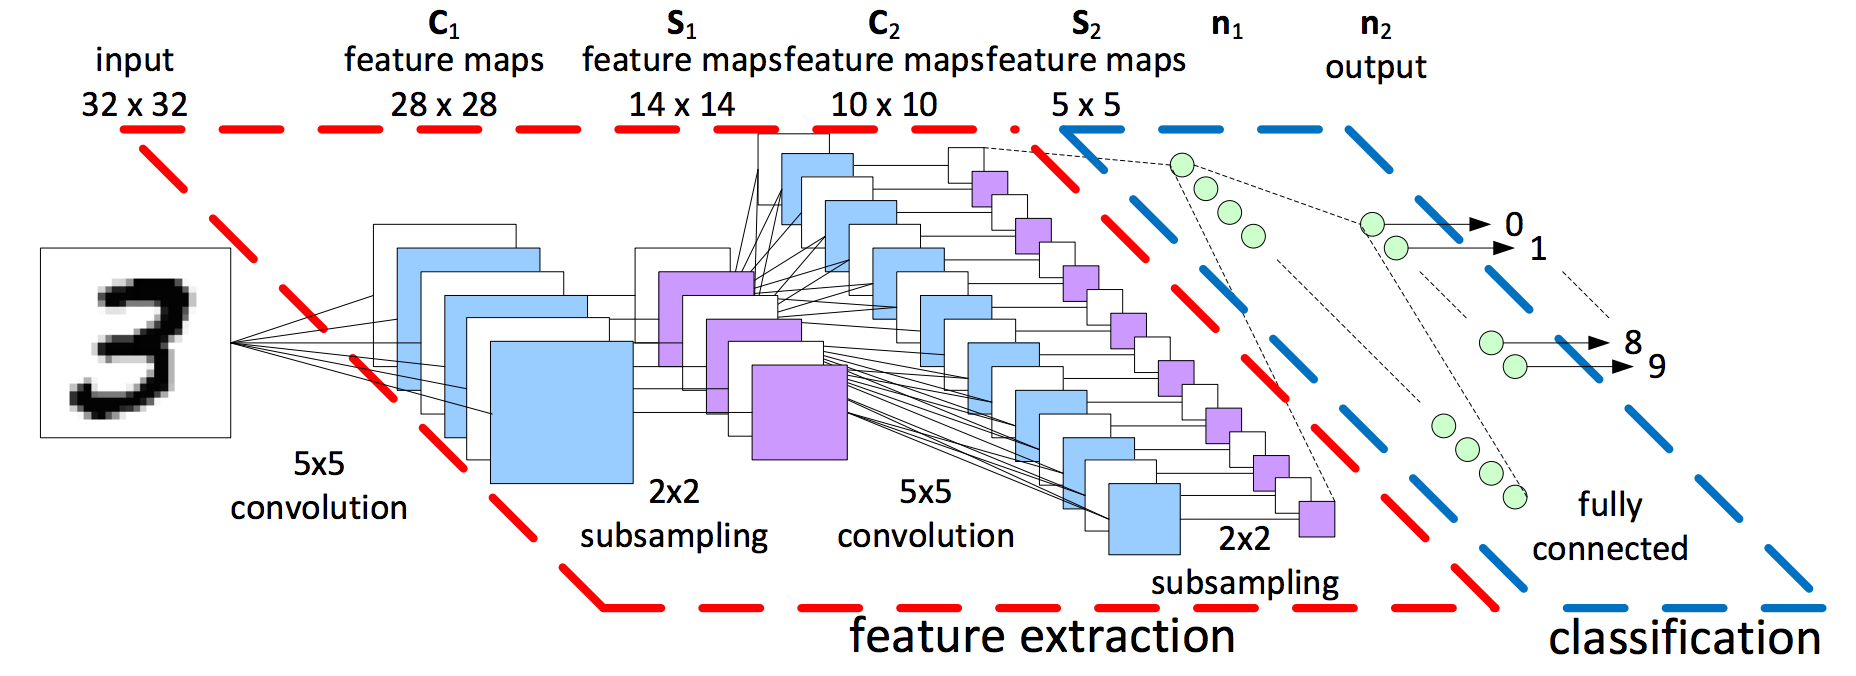
\includegraphics[width=.9\linewidth]{cl_im.png}
\end{center}
\end{frame}


\begin{frame}{Обычно хочется другого}
	\begin{center}
		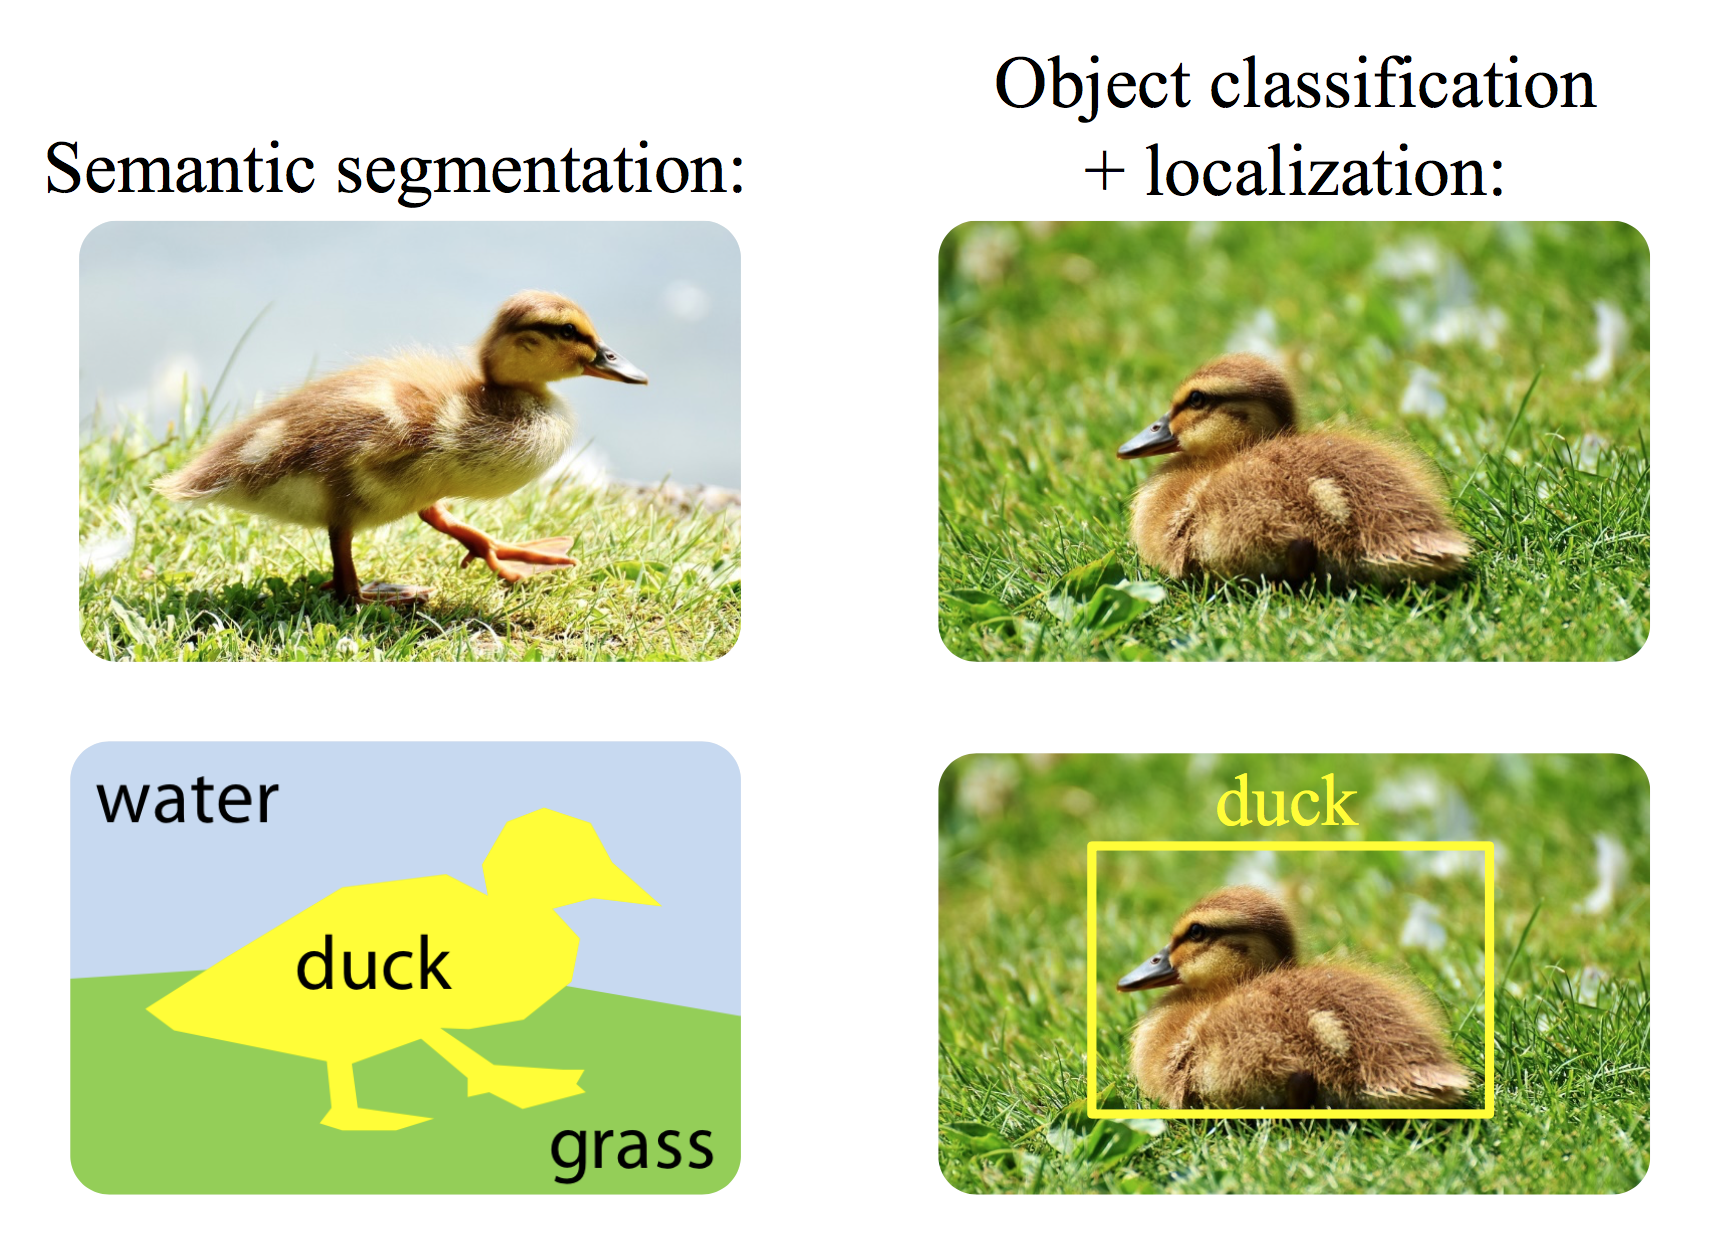
\includegraphics[width=.6\linewidth]{duck.png}
		\vfill 
		{\Large \alert{Мы будем сводить эти задачи к классификации} }
	\end{center}
\end{frame}

\begin{frame}{ Semantic vs. Instance segmentation}
	\begin{center}
		\includegraphics[width=.9\linewidth]{sem_in_seg.png}
	\end{center}
\end{frame}

\begin{frame}{Популярные датасеты}
	\begin{wideitemize}
		\item {\color{blue} \href{https://paperswithcode.com/dataset/pascal-voc}{ Pascal VOC (Visual Object Classes)}}, 20 classes
		\item {\color{blue} \href{https://cocodataset.org/}{MS COCO (Microsoft Common Objects in Context)}}, 91 classes 
		\item ImageNet, 200 classes
		\item Cityscapes, 30 classes
	\end{wideitemize}
\end{frame}


 \begin{transitionframe}
	\begin{center}
		\Huge Детекция объектов (локализация)
	\end{center}
\end{transitionframe}


\begin{frame}{Детекция объектов (локализация)}
	\begin{center}
		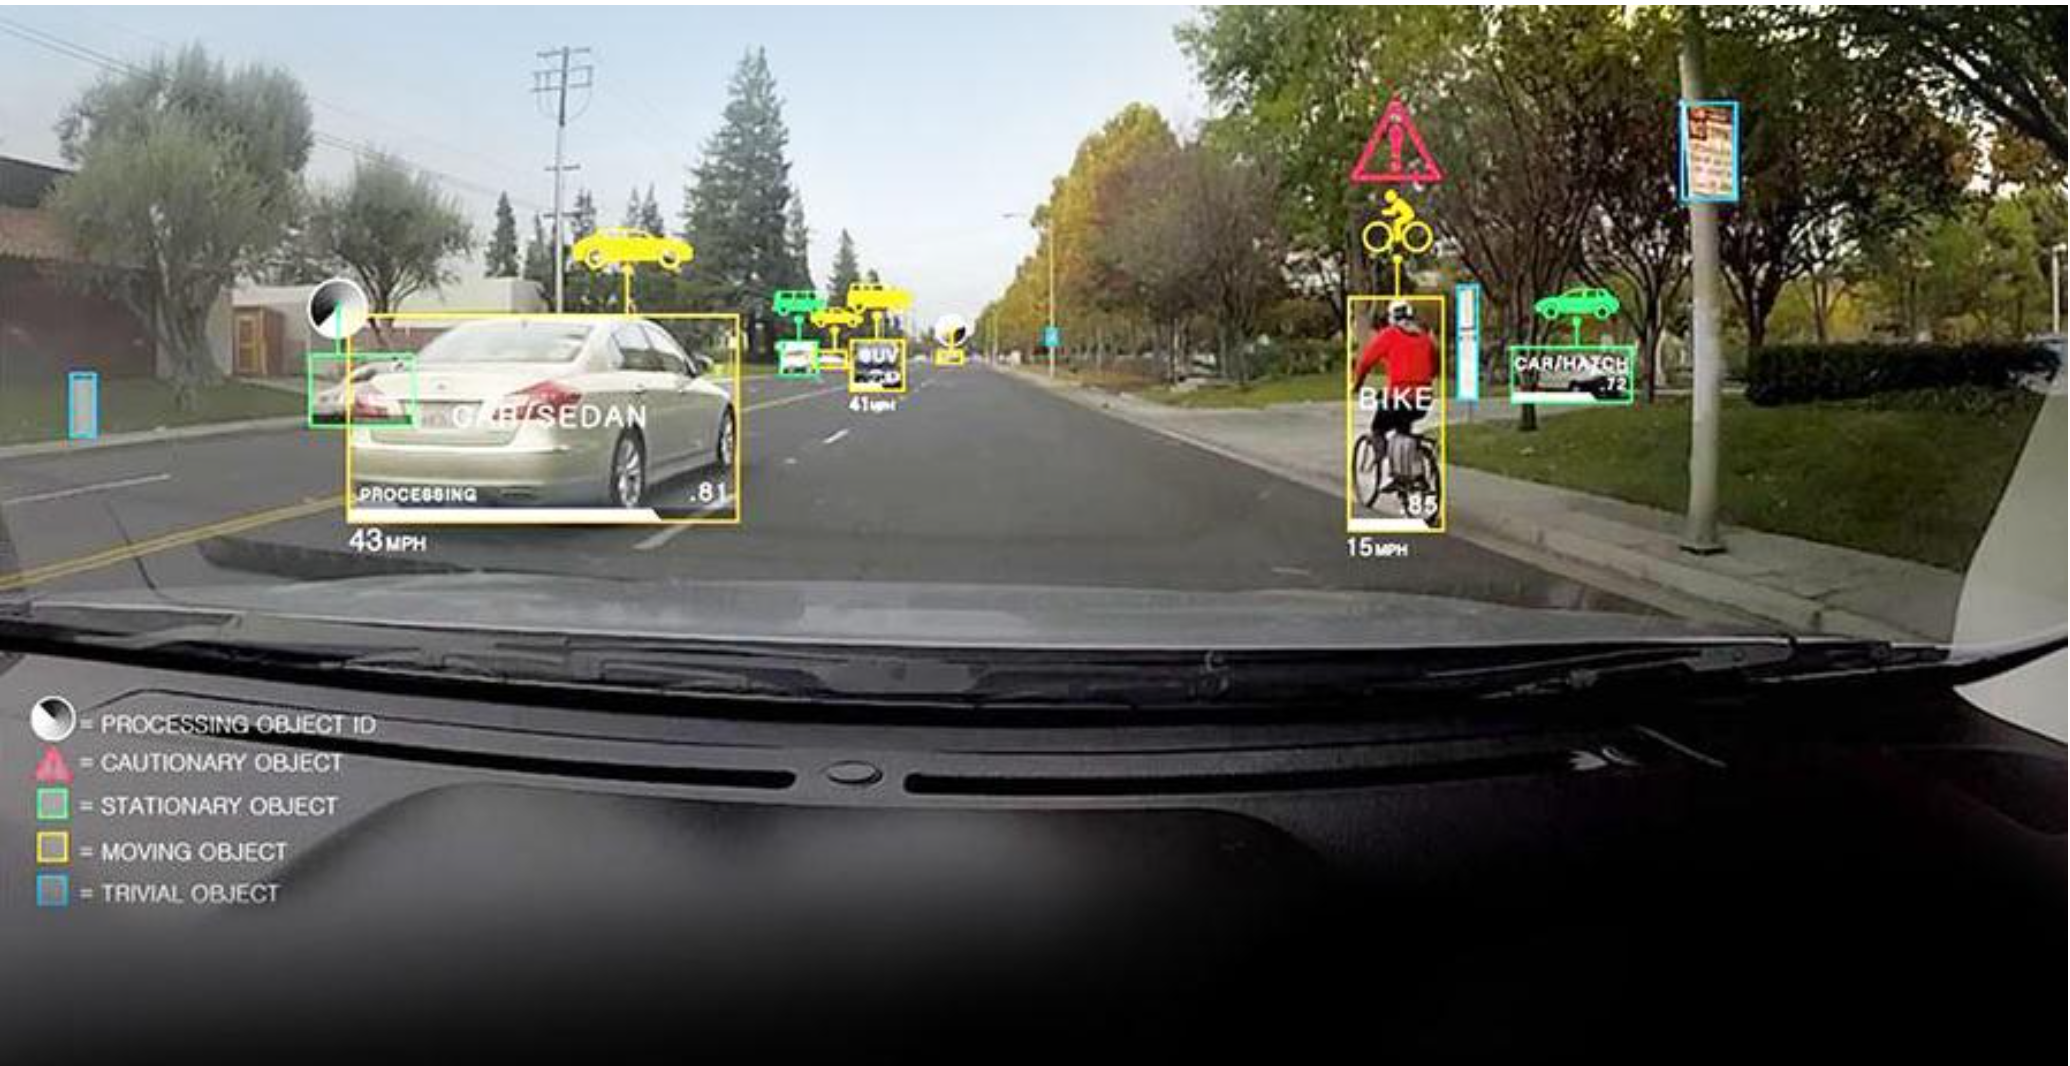
\includegraphics[width=.9\linewidth]{loc2.png}
	\end{center}
\end{frame}

\begin{frame}{Проблемы}
	\begin{wideitemize}
		\item Разное количество объектов на картинке
		\item Большое разнообразие классов
		\item Много редких классов
		\item Хочется, чтобы модель работала быстро и находила объекты в риалтайме (камера)
	\end{wideitemize}
\end{frame}


\begin{frame}{Детекция объектов (локализация)}
	\begin{center}
		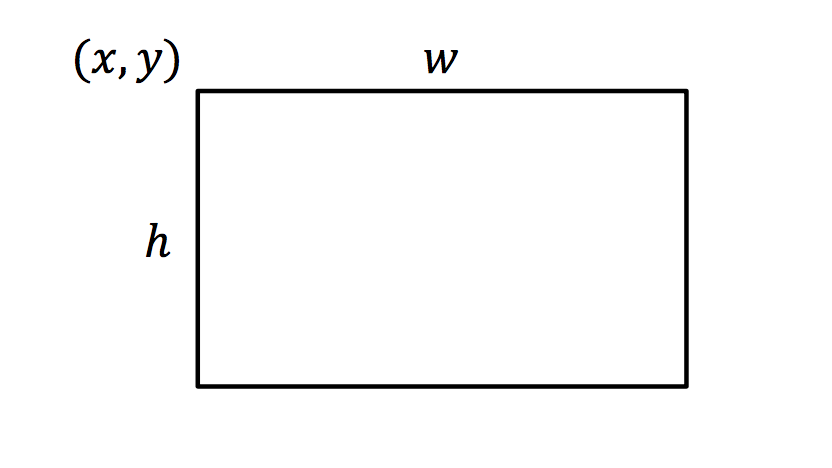
\includegraphics[width=.5\linewidth]{box.png}
	\end{center}
	\begin{itemize}
		\item для локализации объекта нужно нащупать рамочку, в котором он находится
		\item рамочка описывается параметрами $(x,y,w,h)$
	\end{itemize}
\end{frame}


\begin{frame}{Детекция объектов (локализация)}
	\begin{center}
		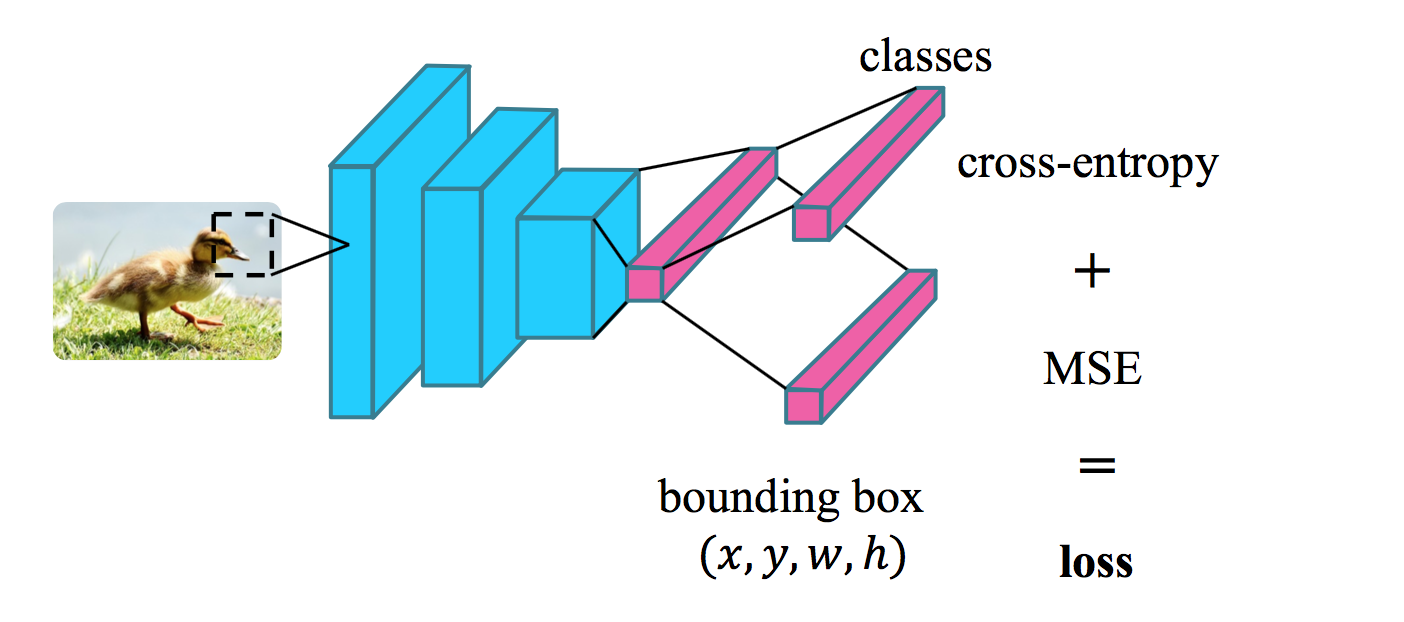
\includegraphics[width=.9\linewidth]{duck_3.png}
	\end{center}
\end{frame}


\begin{frame}{R-CNN (2013)}
	\begin{wideitemize}
		\item Перебирать все прямоугольники очень долго, они могут быть разного размера
		\item Можно сначала генерировать кандидатов в прямоугольники эвристиками, а потом выбирать среди них лучшего
	\end{wideitemize}

	\begin{center}
		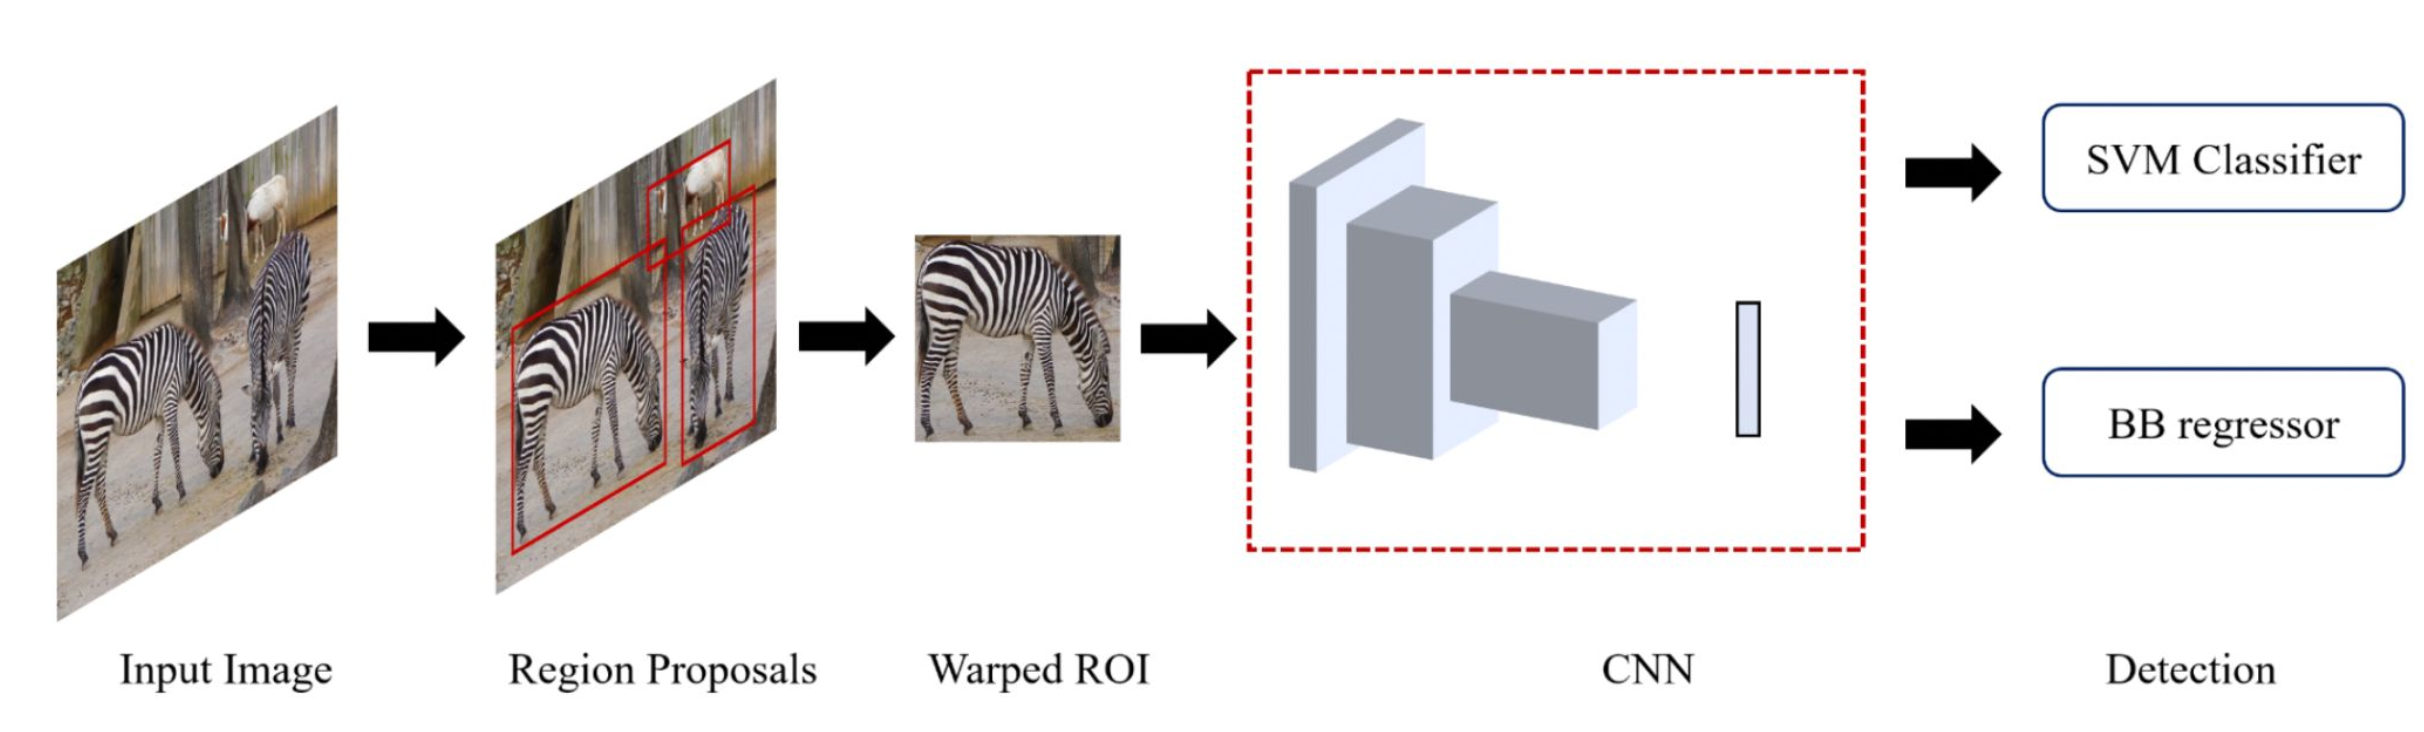
\includegraphics[width=.8\linewidth]{rcnn.png}
	\end{center}

	\vfill
\footnotesize
{\color{blue} \url{https://arxiv.org/abs/1311.2524}} 
\end{frame}


\begin{frame}{Selective Search (2012)}
	
	\begin{center}
		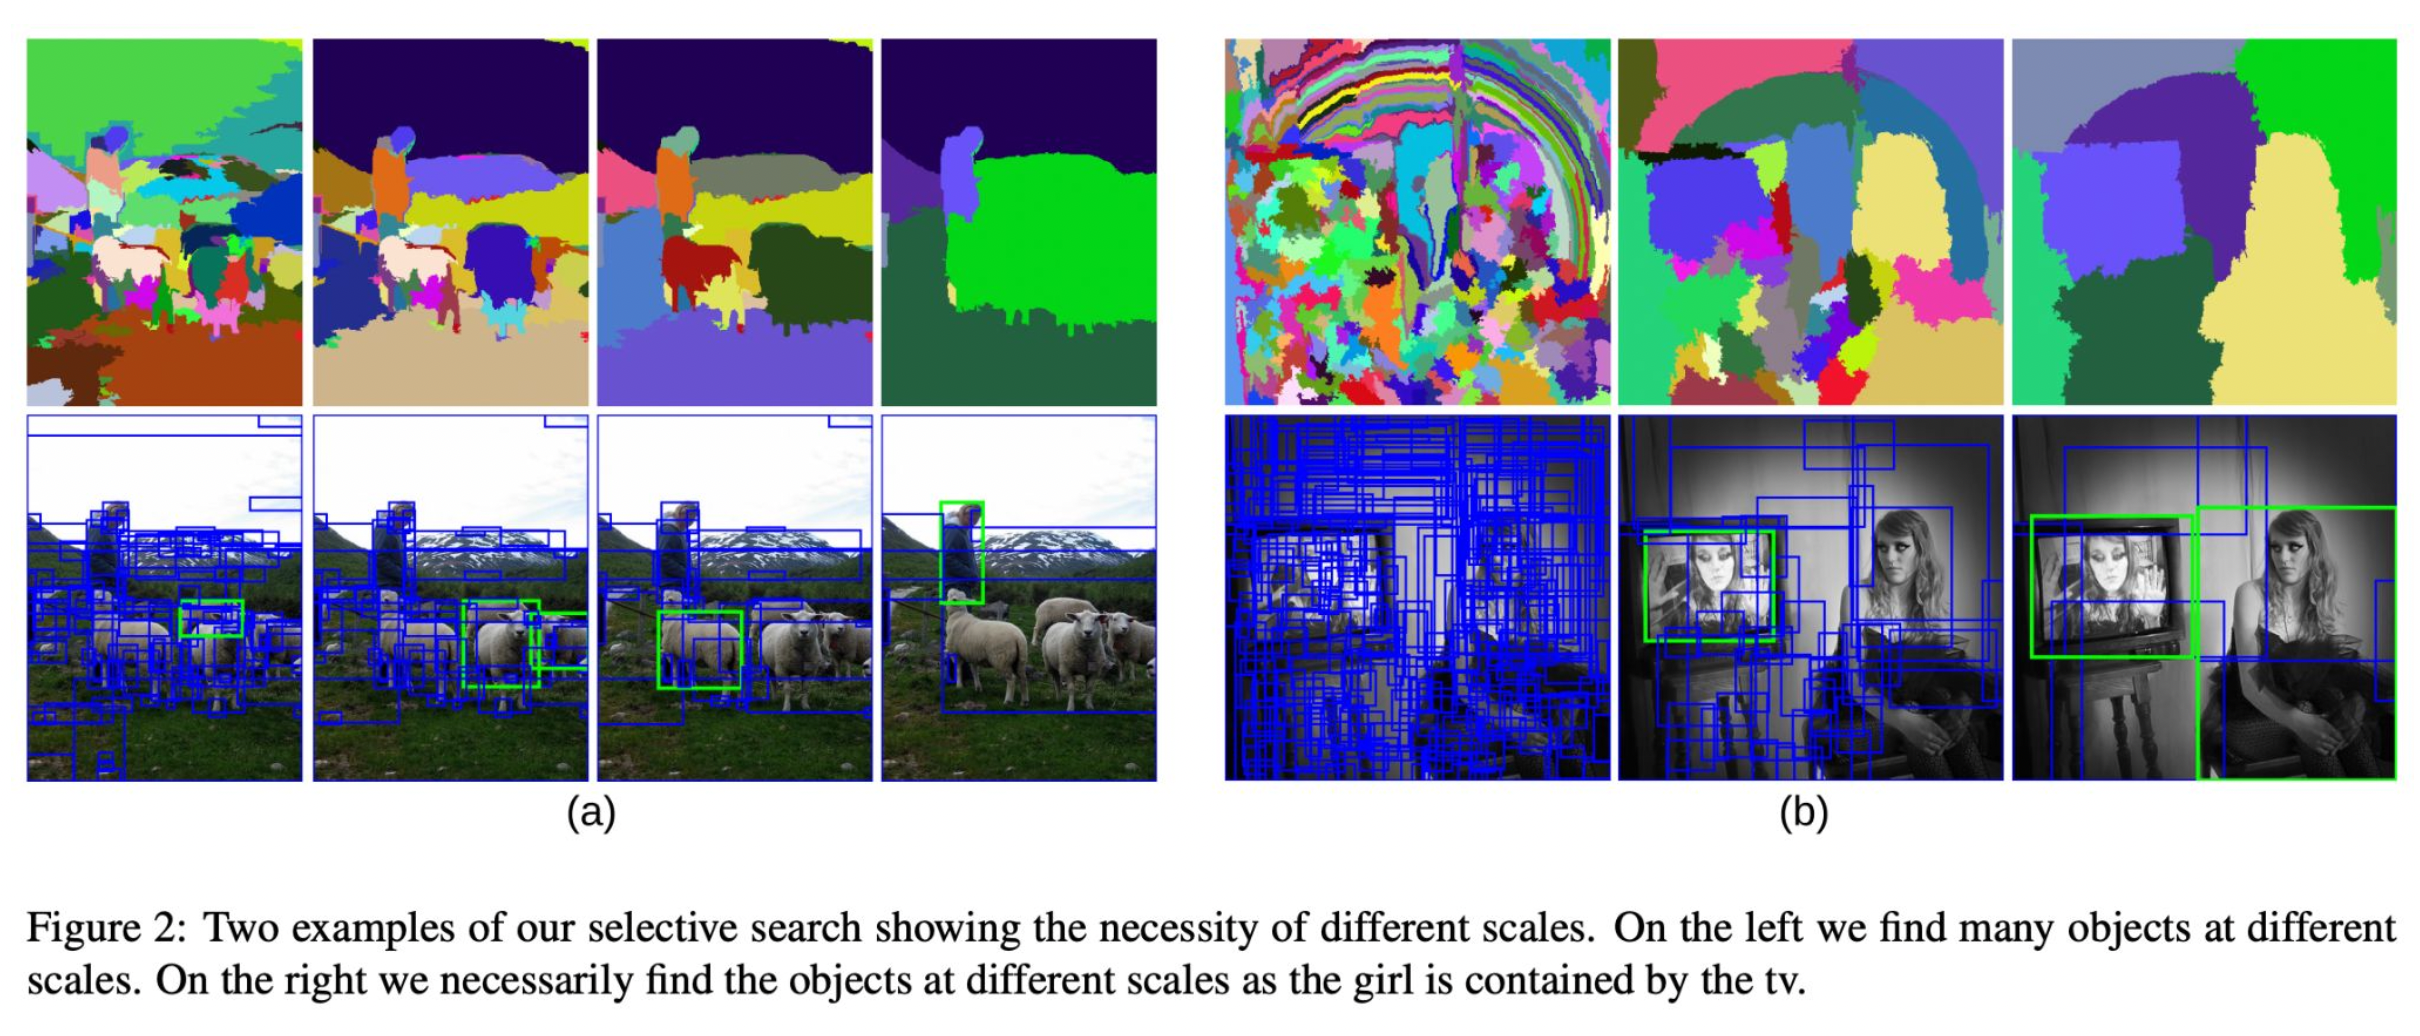
\includegraphics[width=.99\linewidth]{selective_search.png}
	\end{center}
	
	\vfill
	\footnotesize
	{\color{blue} \url{https://ivi.fnwi.uva.nl/isis/publications/2013/UijlingsIJCV2013/UijlingsIJCV2013.pdf}}
\end{frame}


\begin{frame}{Non-maximum suppression (NMS)}
	\begin{wideitemize}
		\item Сгенерируем много прямоугольников для одного и того же объекта
		\item Оставим самый классный (например с наибольшим IoU)
	\end{wideitemize}	

	\begin{center}
		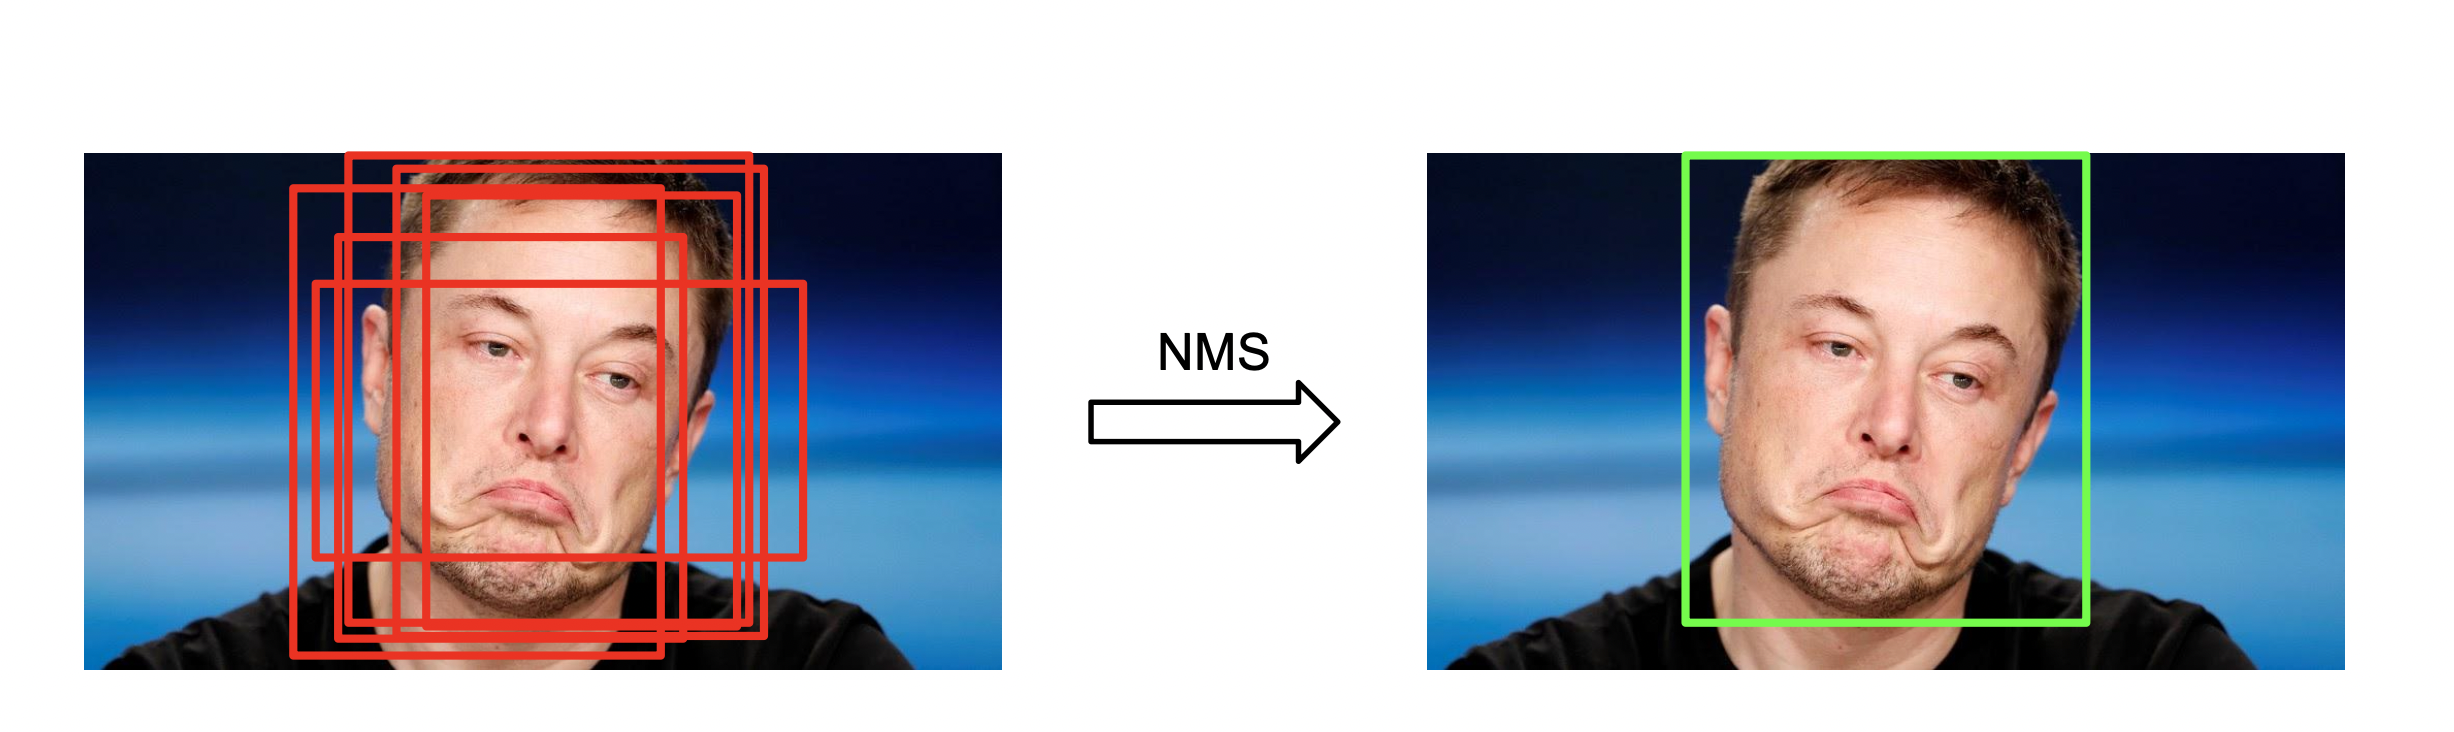
\includegraphics[width=.99\linewidth]{nms.png}
	\end{center}
	\vfill
	\footnotesize
	{\color{blue} \url{https://ivi.fnwi.uva.nl/isis/publications/2013/UijlingsIJCV2013/UijlingsIJCV2013.pdf}}
\end{frame}

 \begin{frame}{Проблемы RCNN}
 	\begin{wideitemize}
 		\item Исторически это самая первая моделька
 		\item Перебирать все прямоугольники очень долго (2000 per image в оригинальной статье)
 		\item Нейросетка долго обучается и применяется  (~47 seconds/image)
 		\item Для поиска интересных частей картинки используются эвристики 
 		\item \alert{Хочется всё это дело ускорить}
 	\end{wideitemize}
 \end{frame}


\begin{frame}{Mean average precision}
\begin{center}
	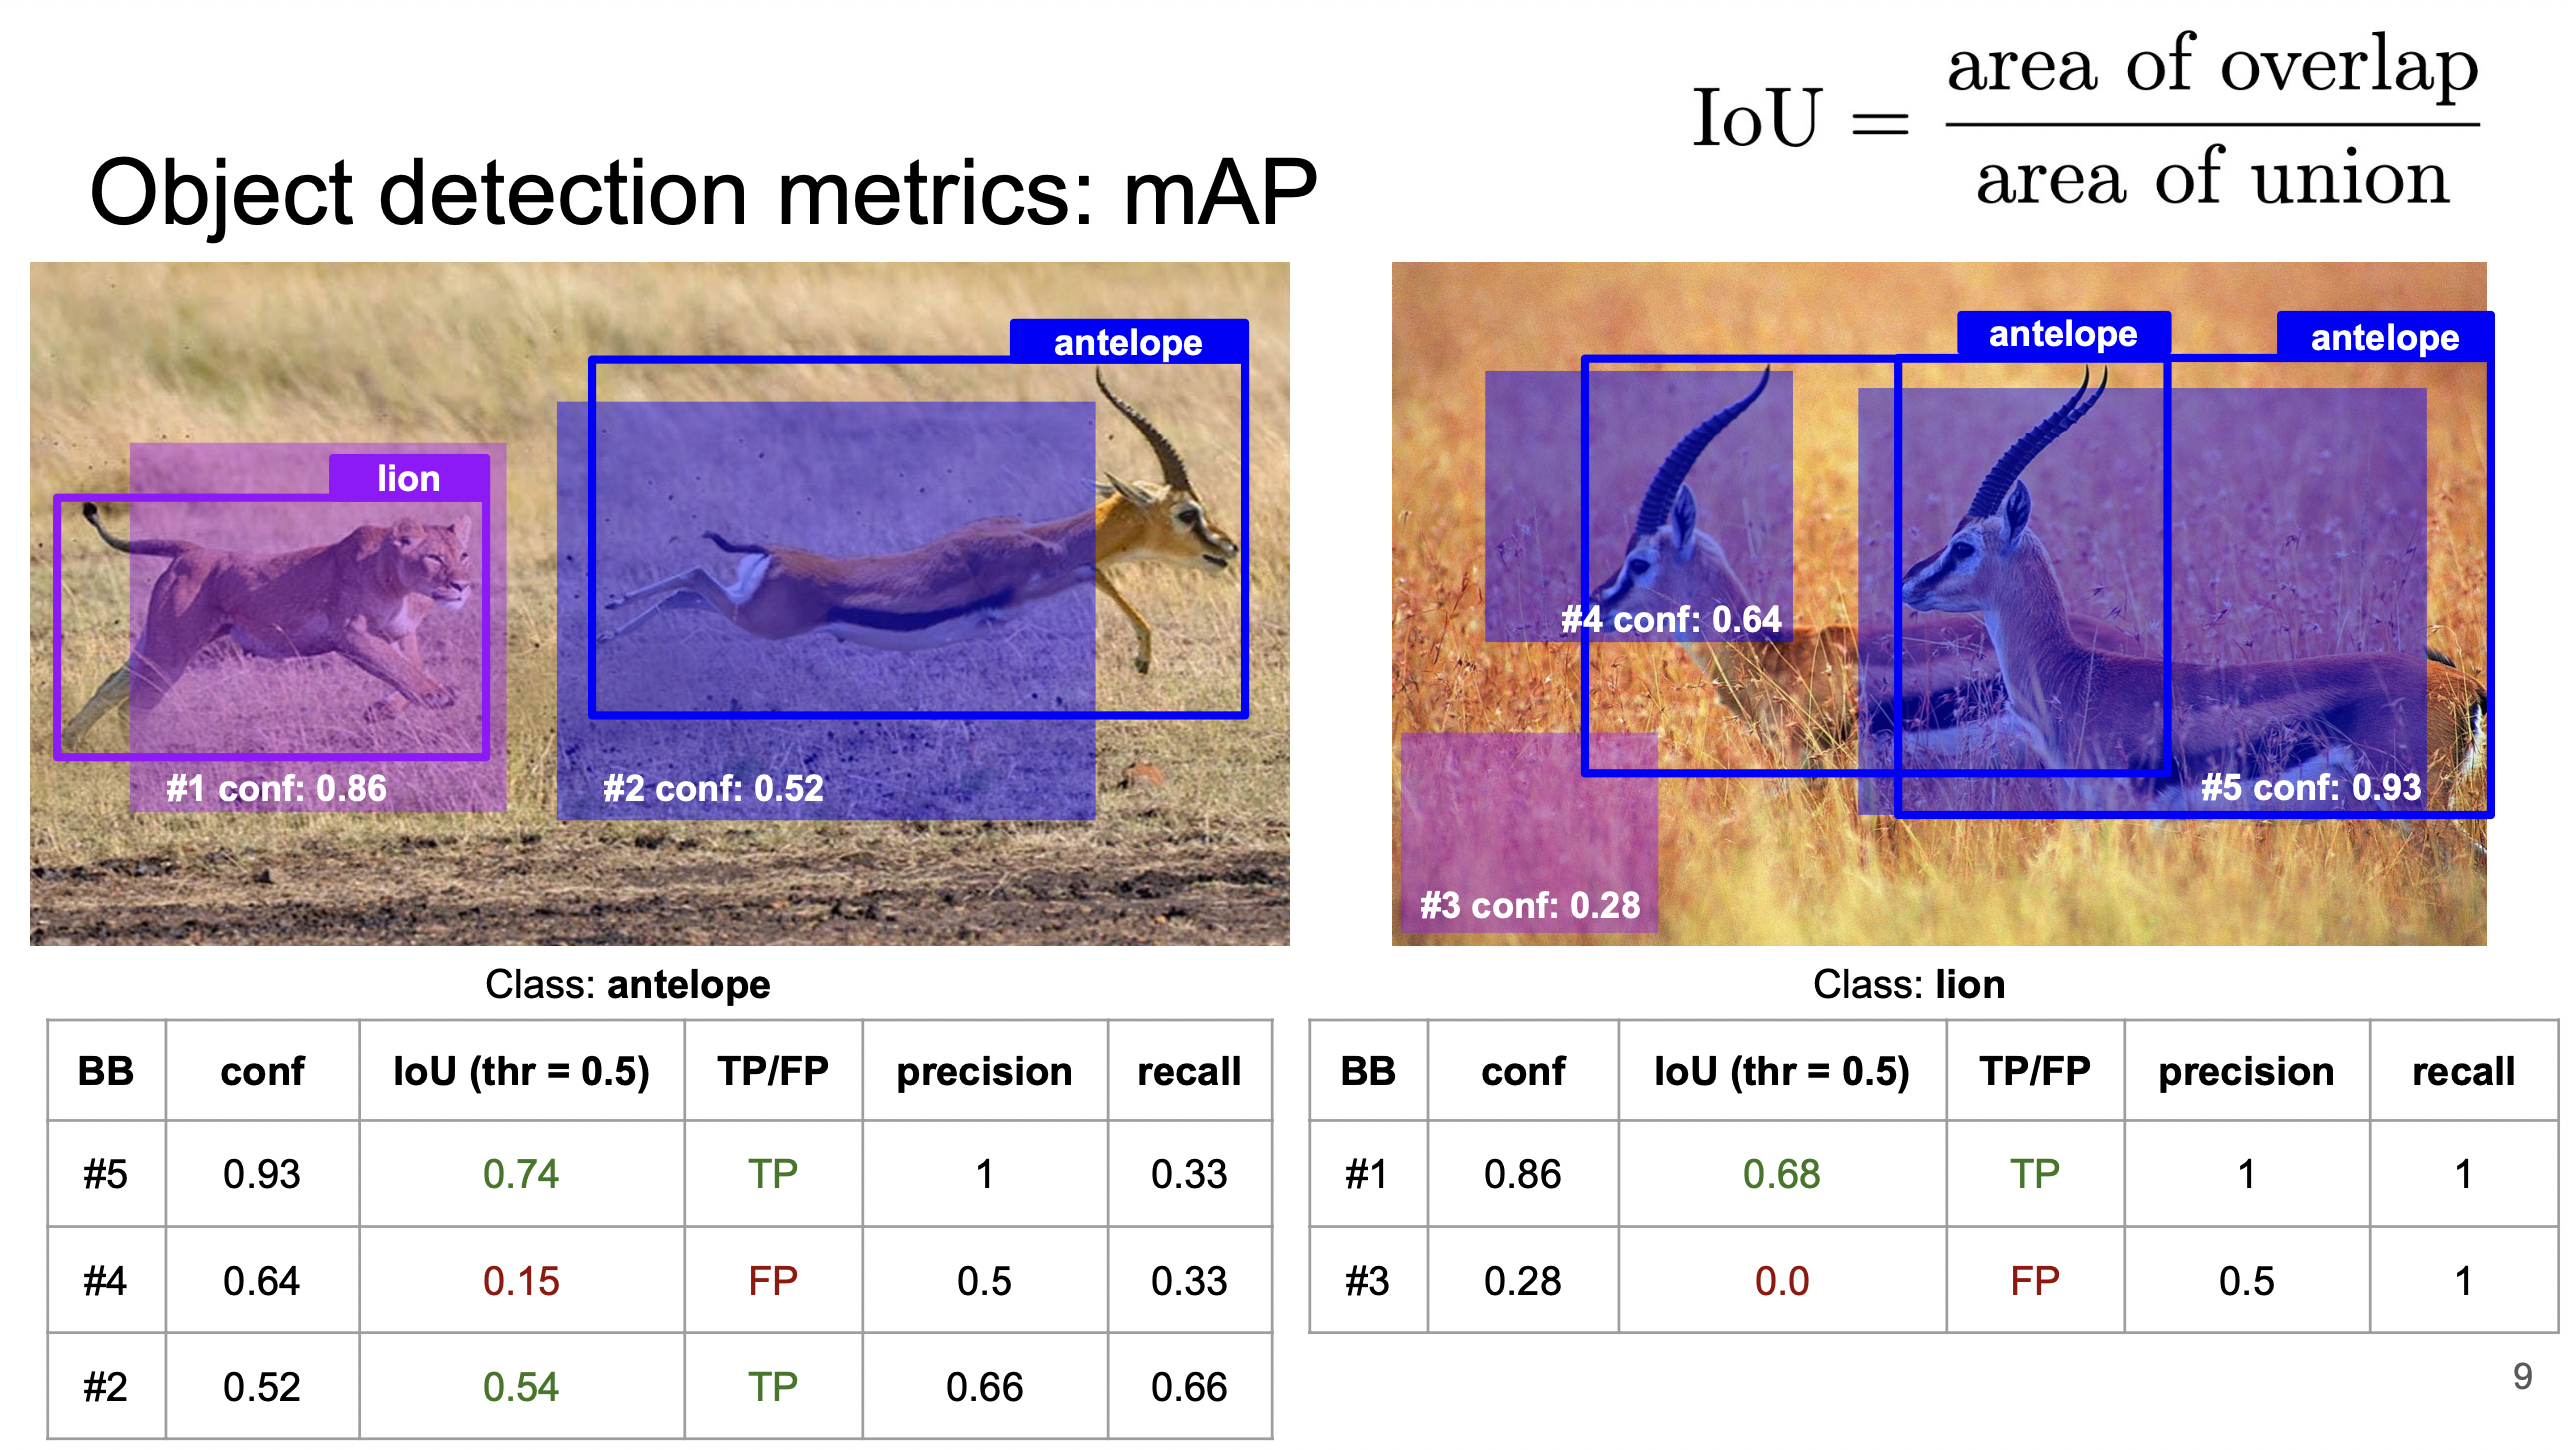
\includegraphics[width=.9\linewidth]{map.png}
\end{center}
\end{frame}


\begin{frame}{Fast R-CNN (2015)}
\begin{wideitemize}
	\item Давайте перебирать прямоугольники не на исходной картинке, а на карте признаков
	\item Добавим слой RoI (Region of Interest) pooling
	\item Получаем сильное ускорение работы
\end{wideitemize}	
	\begin{center}
		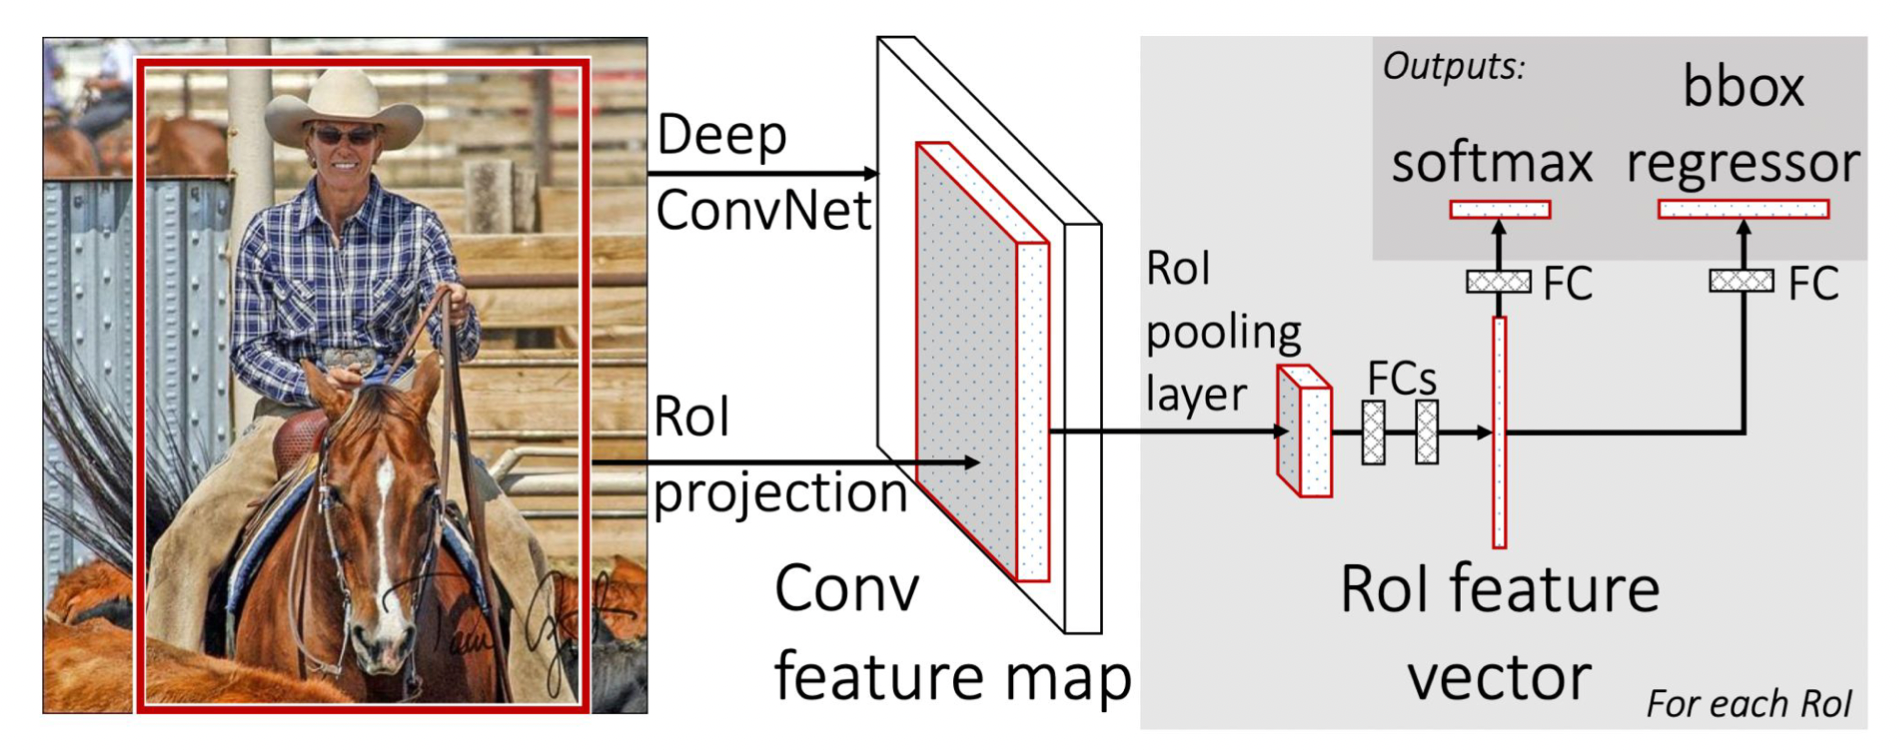
\includegraphics[width=.7\linewidth]{fast_rcnn.png}
	\end{center}
	
	\vfill
	\footnotesize
	{\color{blue} \url{https://arxiv.org/abs/1504.08083}} 
\end{frame}


\begin{frame}{Region of Interest (RoI) pooling}
	\begin{columns}[T] % align columns
		\begin{column}{.49\textwidth}
			\begin{wideitemize}	
				\item Берём интересную часть (reion proposal)
				\item Делим на секции (число секций совпадает с размерностью выхода)
				\item К каждой секции применяем max pooling
			\end{wideitemize}
		\end{column}%
		\hfill%
		\begin{column}{.49\textwidth}
			\begin{center}
				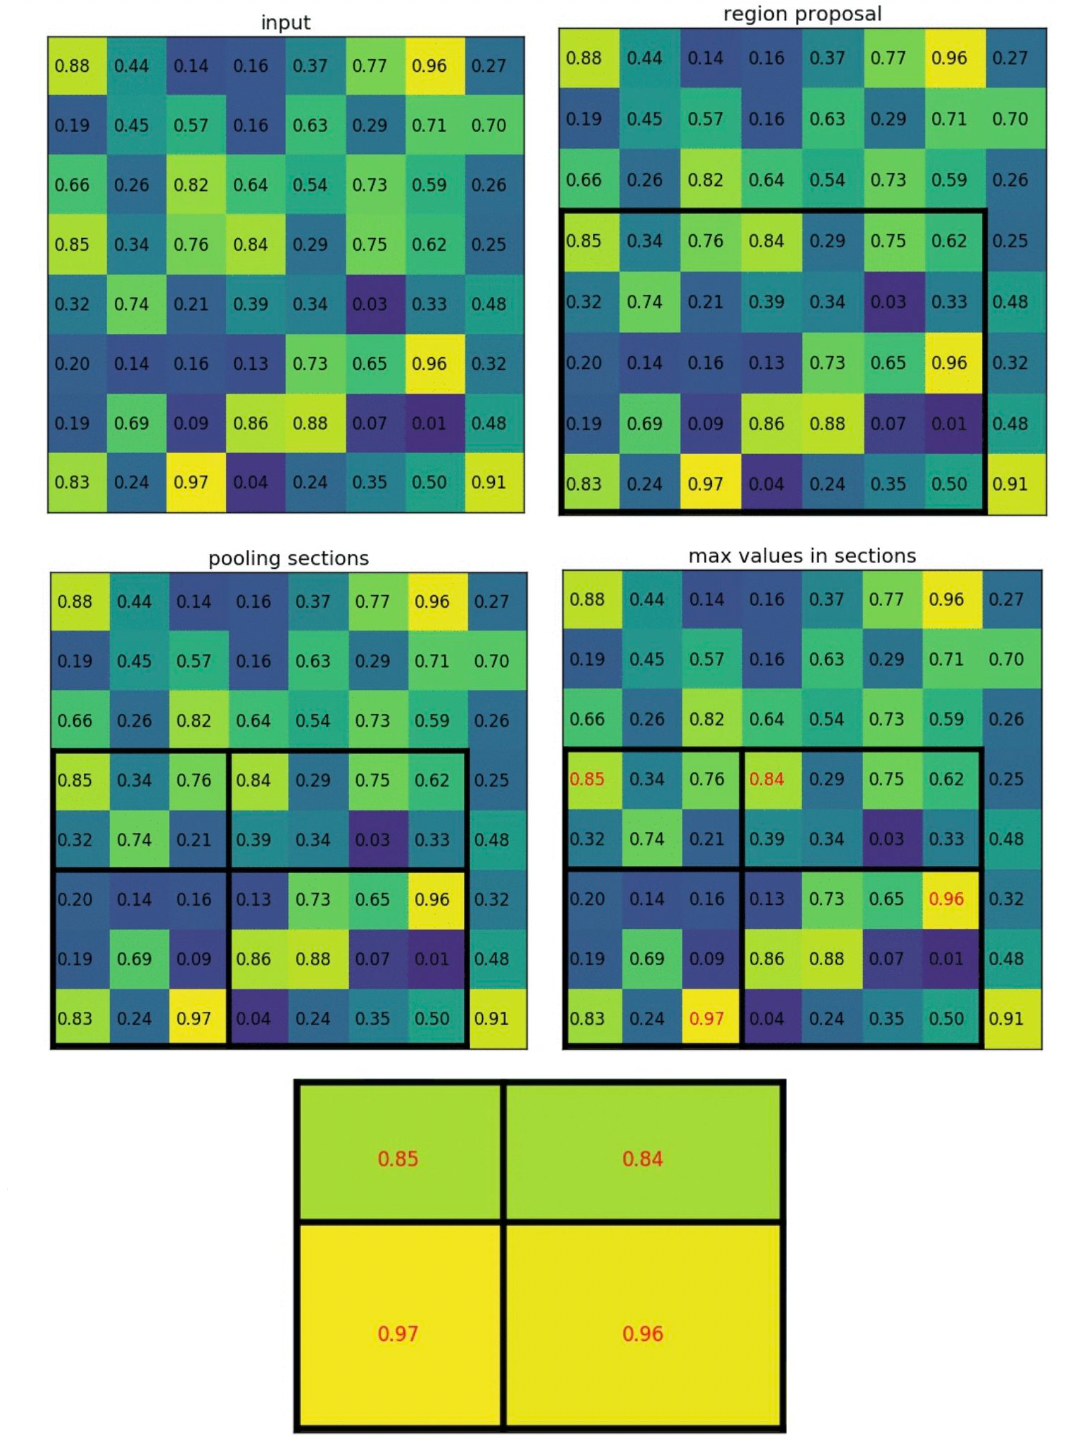
\includegraphics[width=.7\linewidth]{roi.png}
			\end{center}
		\end{column}%
	\end{columns}
\end{frame}


\begin{frame}{Faster R-CNN (2015)}
	\begin{columns}[T] % align columns
		\begin{column}{.49\textwidth}
			\begin{wideitemize}	
				\item Будем искать зоны под прямоугольники с помощью нейросети Region Proposal Network вместо Selective Search
			\end{wideitemize}
		\vspace{2mm}
		\begin{center}
			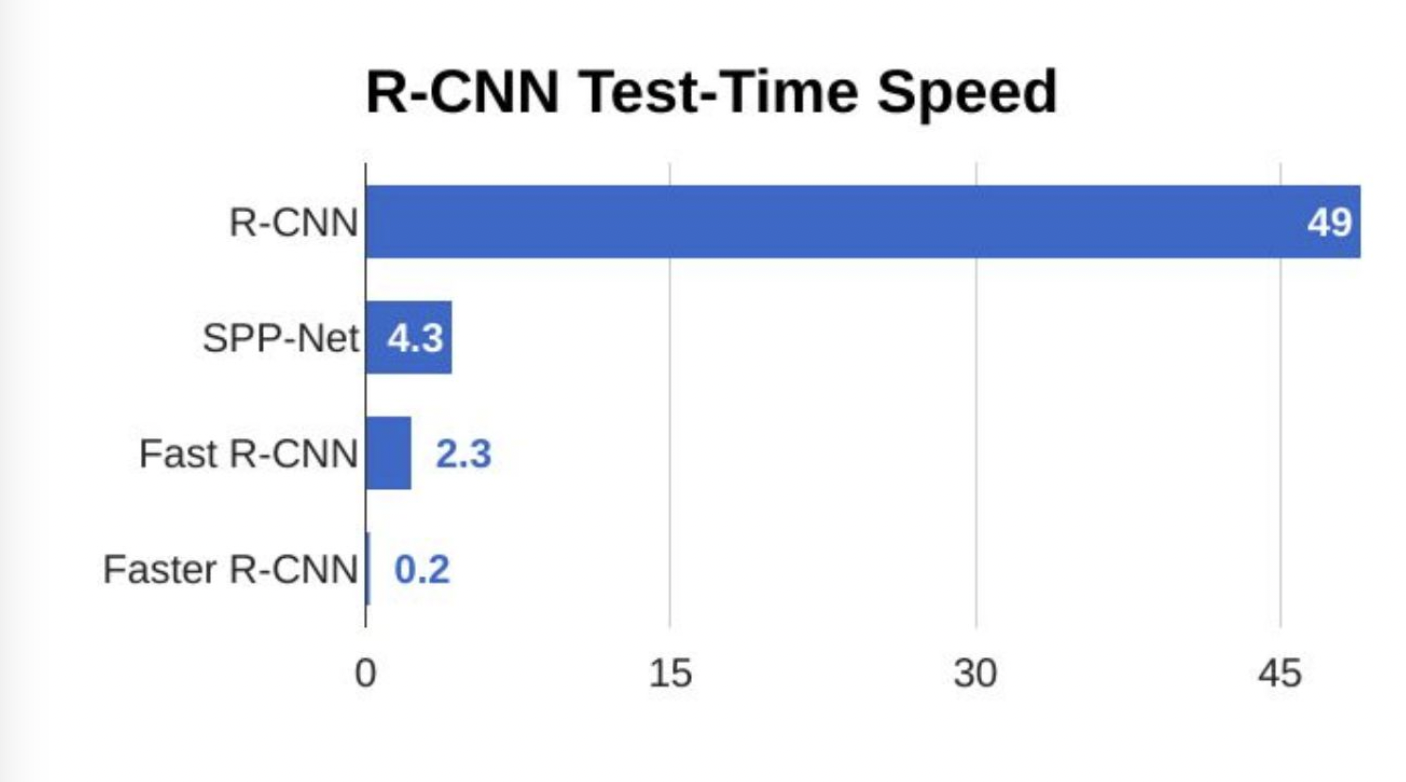
\includegraphics[width=.95\linewidth]{rcnn_speed.png}
		\end{center}
		\end{column}%
		\hfill%
		\begin{column}{.49\textwidth}
			\begin{center}
				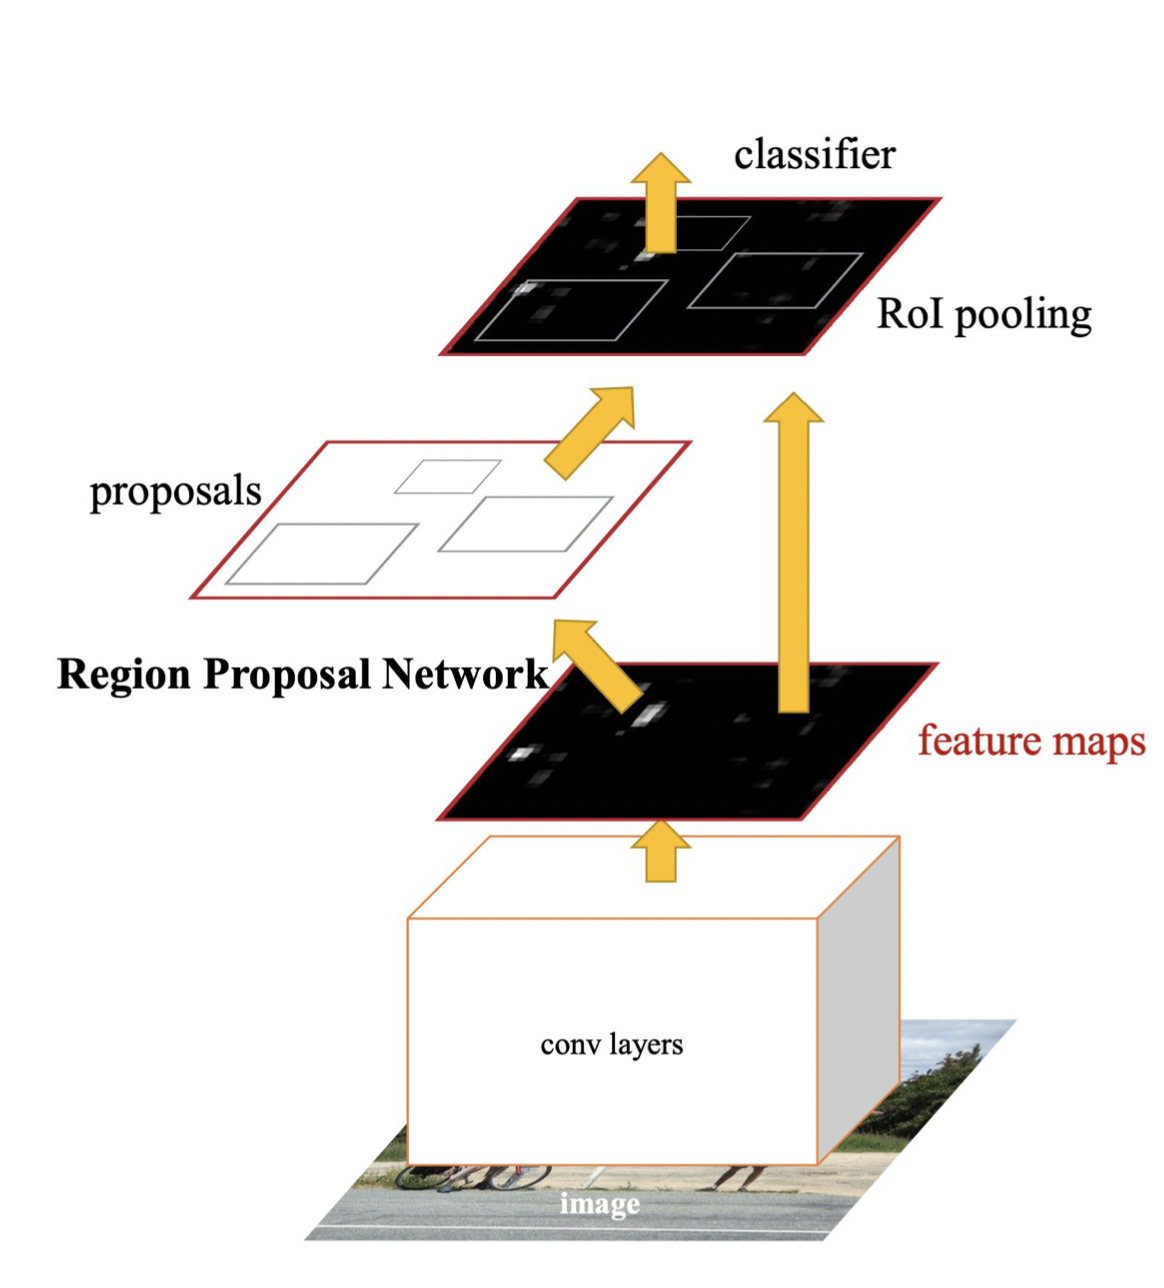
\includegraphics[width=.8\linewidth]{faster_rcnn.png}
			\end{center}
		\end{column}%
	\end{columns}
	\vfill
\footnotesize
{\color{blue} \url{https://arxiv.org/abs/1506.01497}} 
\end{frame}


\begin{frame}{ YOLO (2015)}
	\begin{columns}[T] % align columns
	\begin{column}{.35\textwidth}
		\begin{wideitemize}	
			\item Мы сначала искали регионы интереса, а потом обрабатывали их
			\item Одновременный поиск кандидатов и определение их классов (YOLO, you only look once)
		\end{wideitemize}
	\end{column}%
	\hfill%
	\begin{column}{.65\textwidth}
		\begin{center}
			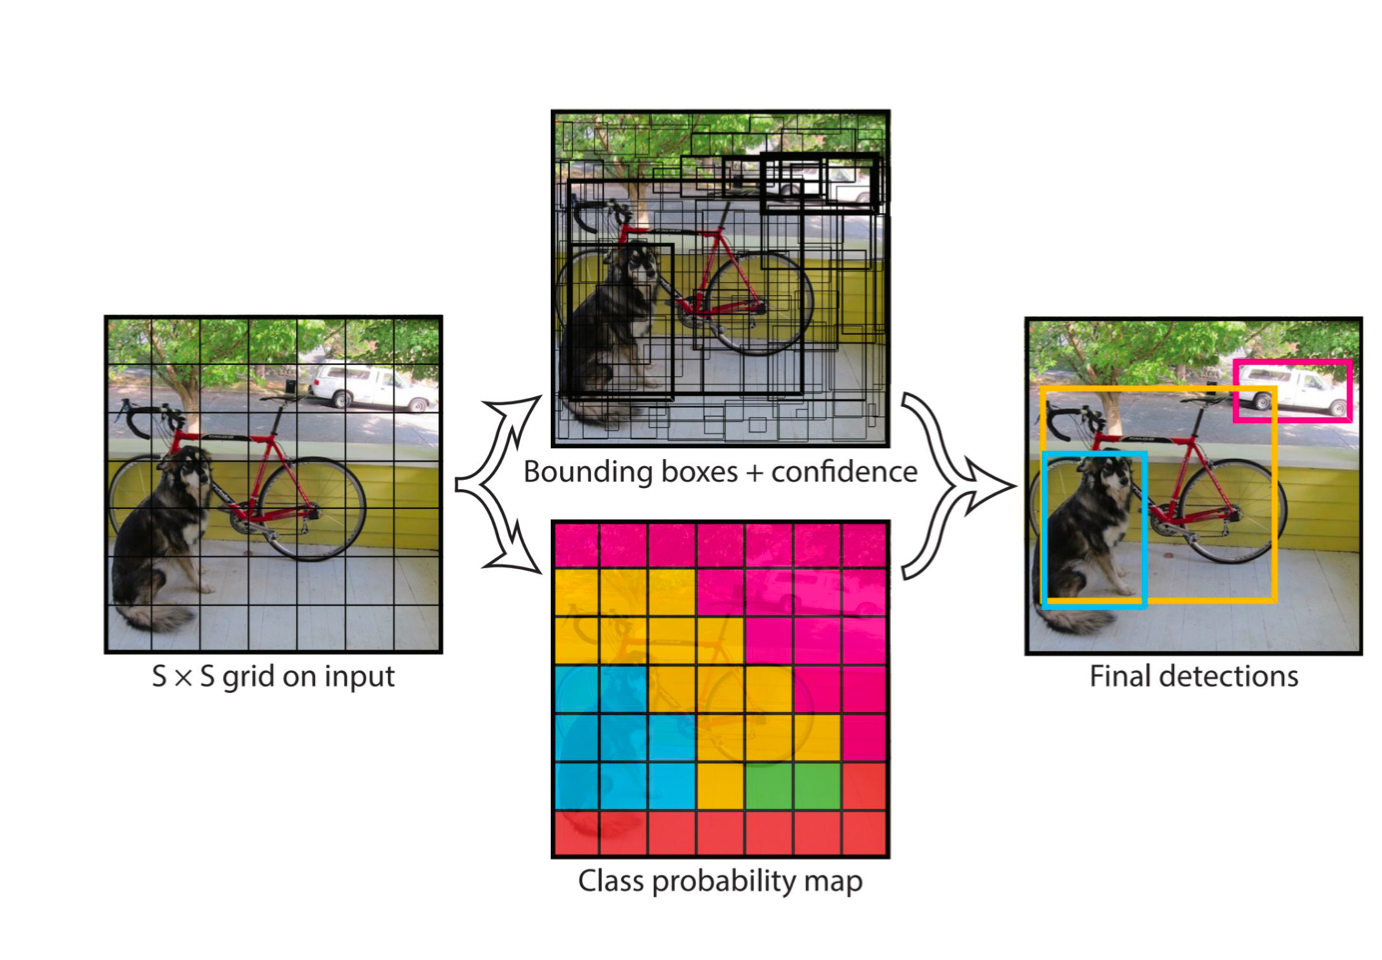
\includegraphics[width=.9\linewidth]{yolo.png}
		\end{center} 
	\end{column}%
\end{columns}
	
	\vfill
	\footnotesize
	{\color{blue} \url{https://arxiv.org/abs/1506.02640}} 
\end{frame}

\begin{frame}{ YOLO (2015)}
	\begin{columns}[T] % align columns
		\begin{column}{.59\textwidth}
			\begin{wideitemize}	
				\item You Only Look Once
				\item Делим изображение на ячейки размера  $S \times S$ 
				\item Для каждой ячейки предсказываем $B$ прямоугольников (boundig box)
				\item Одновременно предсказываем для каждой ячейки класс
				\item Применяем NMS и получаем итог
			\end{wideitemize}
		\end{column}%
		\hfill%
		\begin{column}{.39\textwidth}
			\begin{center}
				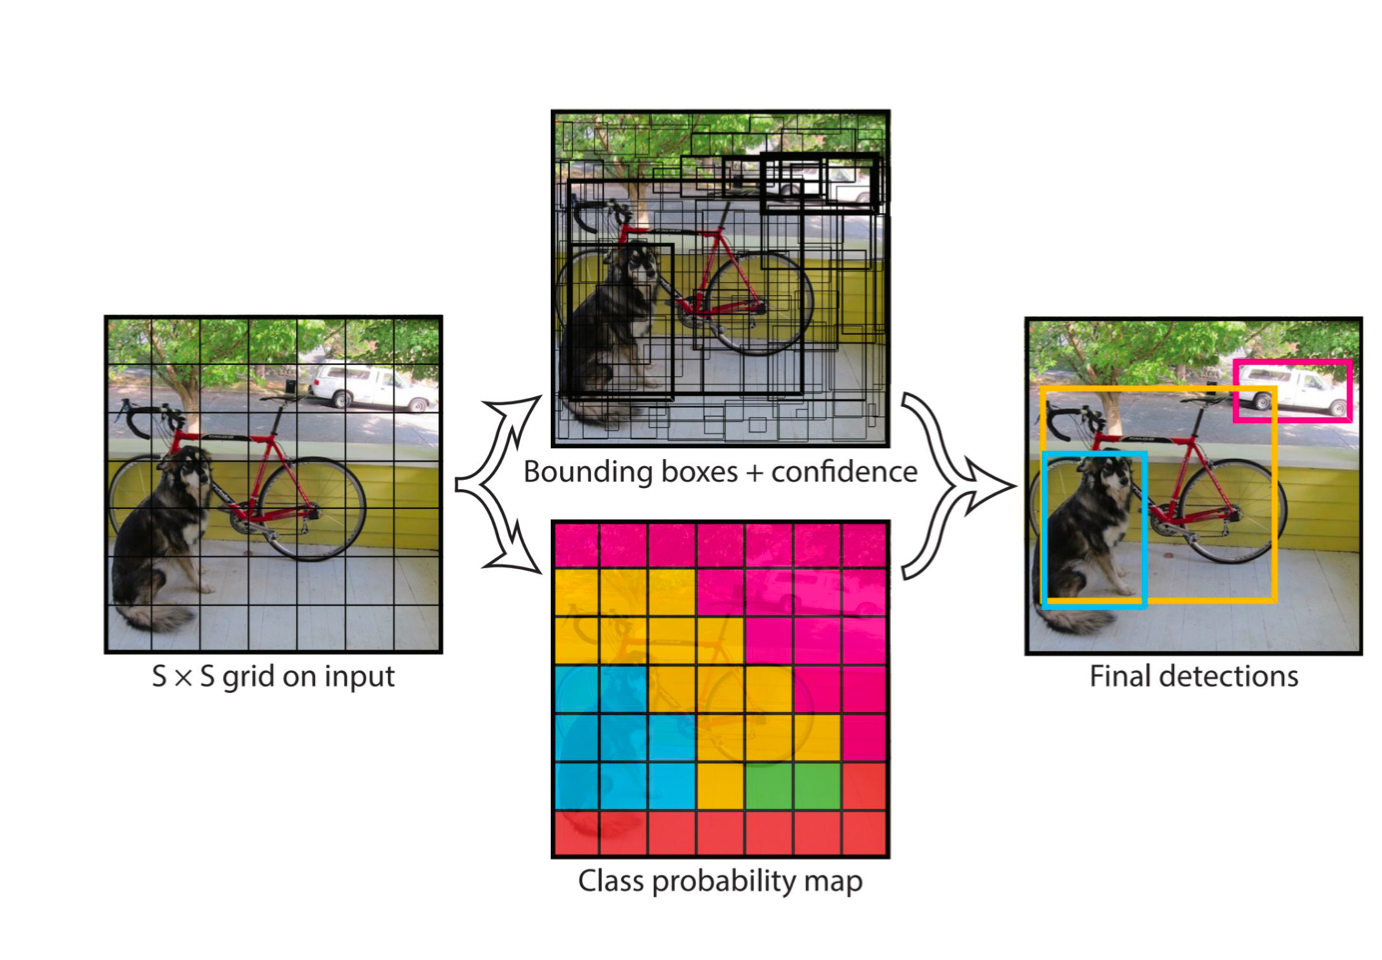
\includegraphics[width=.99\linewidth]{yolo.png}
			\end{center} 
		\end{column}%
	\end{columns}
	\vfill
	\footnotesize
	{\color{blue} \url{https://arxiv.org/abs/1506.02640}} 
\end{frame}


\begin{transitionframe}
	\begin{center}
		\Huge  Семантическая сегментация
	\end{center}
\end{transitionframe}


\begin{frame}{Постановка задачи}
	\begin{center}
		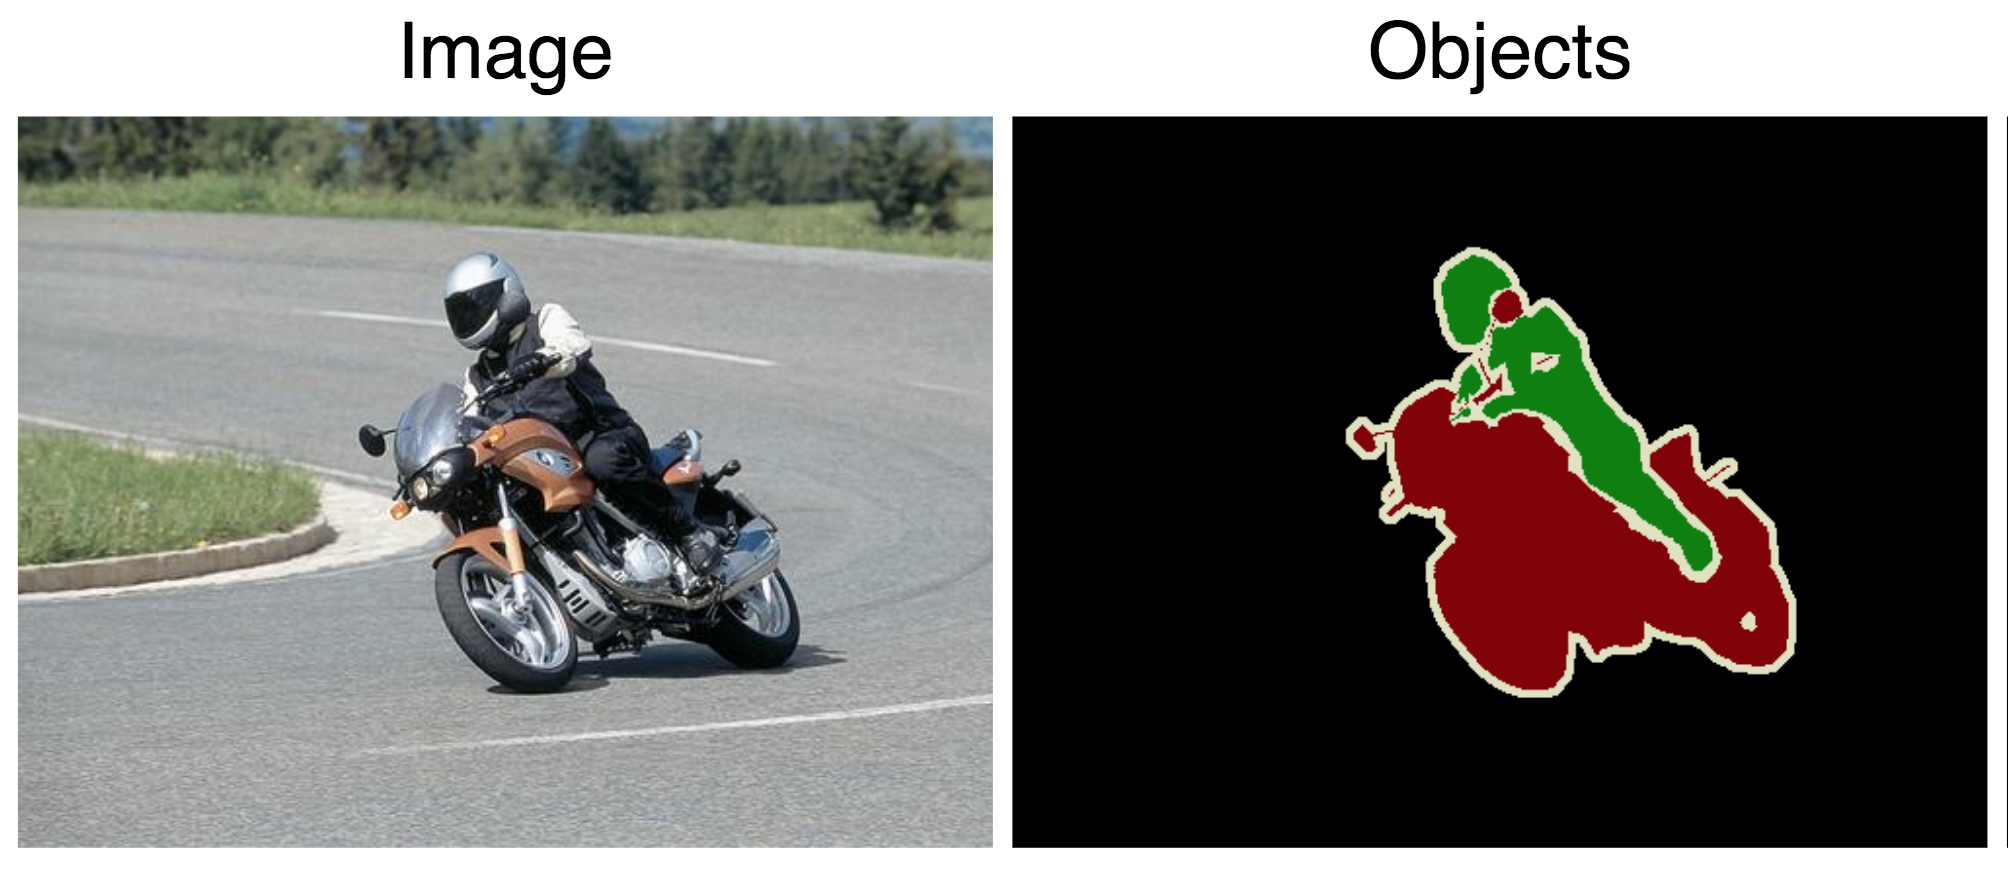
\includegraphics[width=.5\linewidth]{segm_data.png}
	\end{center}
	\begin{itemize}
		\item На вход модели подаются изображения и их корректные сегментации
		\item Каждый объект содержит сильно больше информации, чем при классификации 
		\item Можно обучаться на более маленьких выборках
	\end{itemize}
	\vfill
	\footnotesize
	{\color{blue} \url{http://host.robots.ox.ac.uk/pascal/VOC/voc2012/}} 
\end{frame}


\begin{frame}{Метрики}
	\begin{center}
		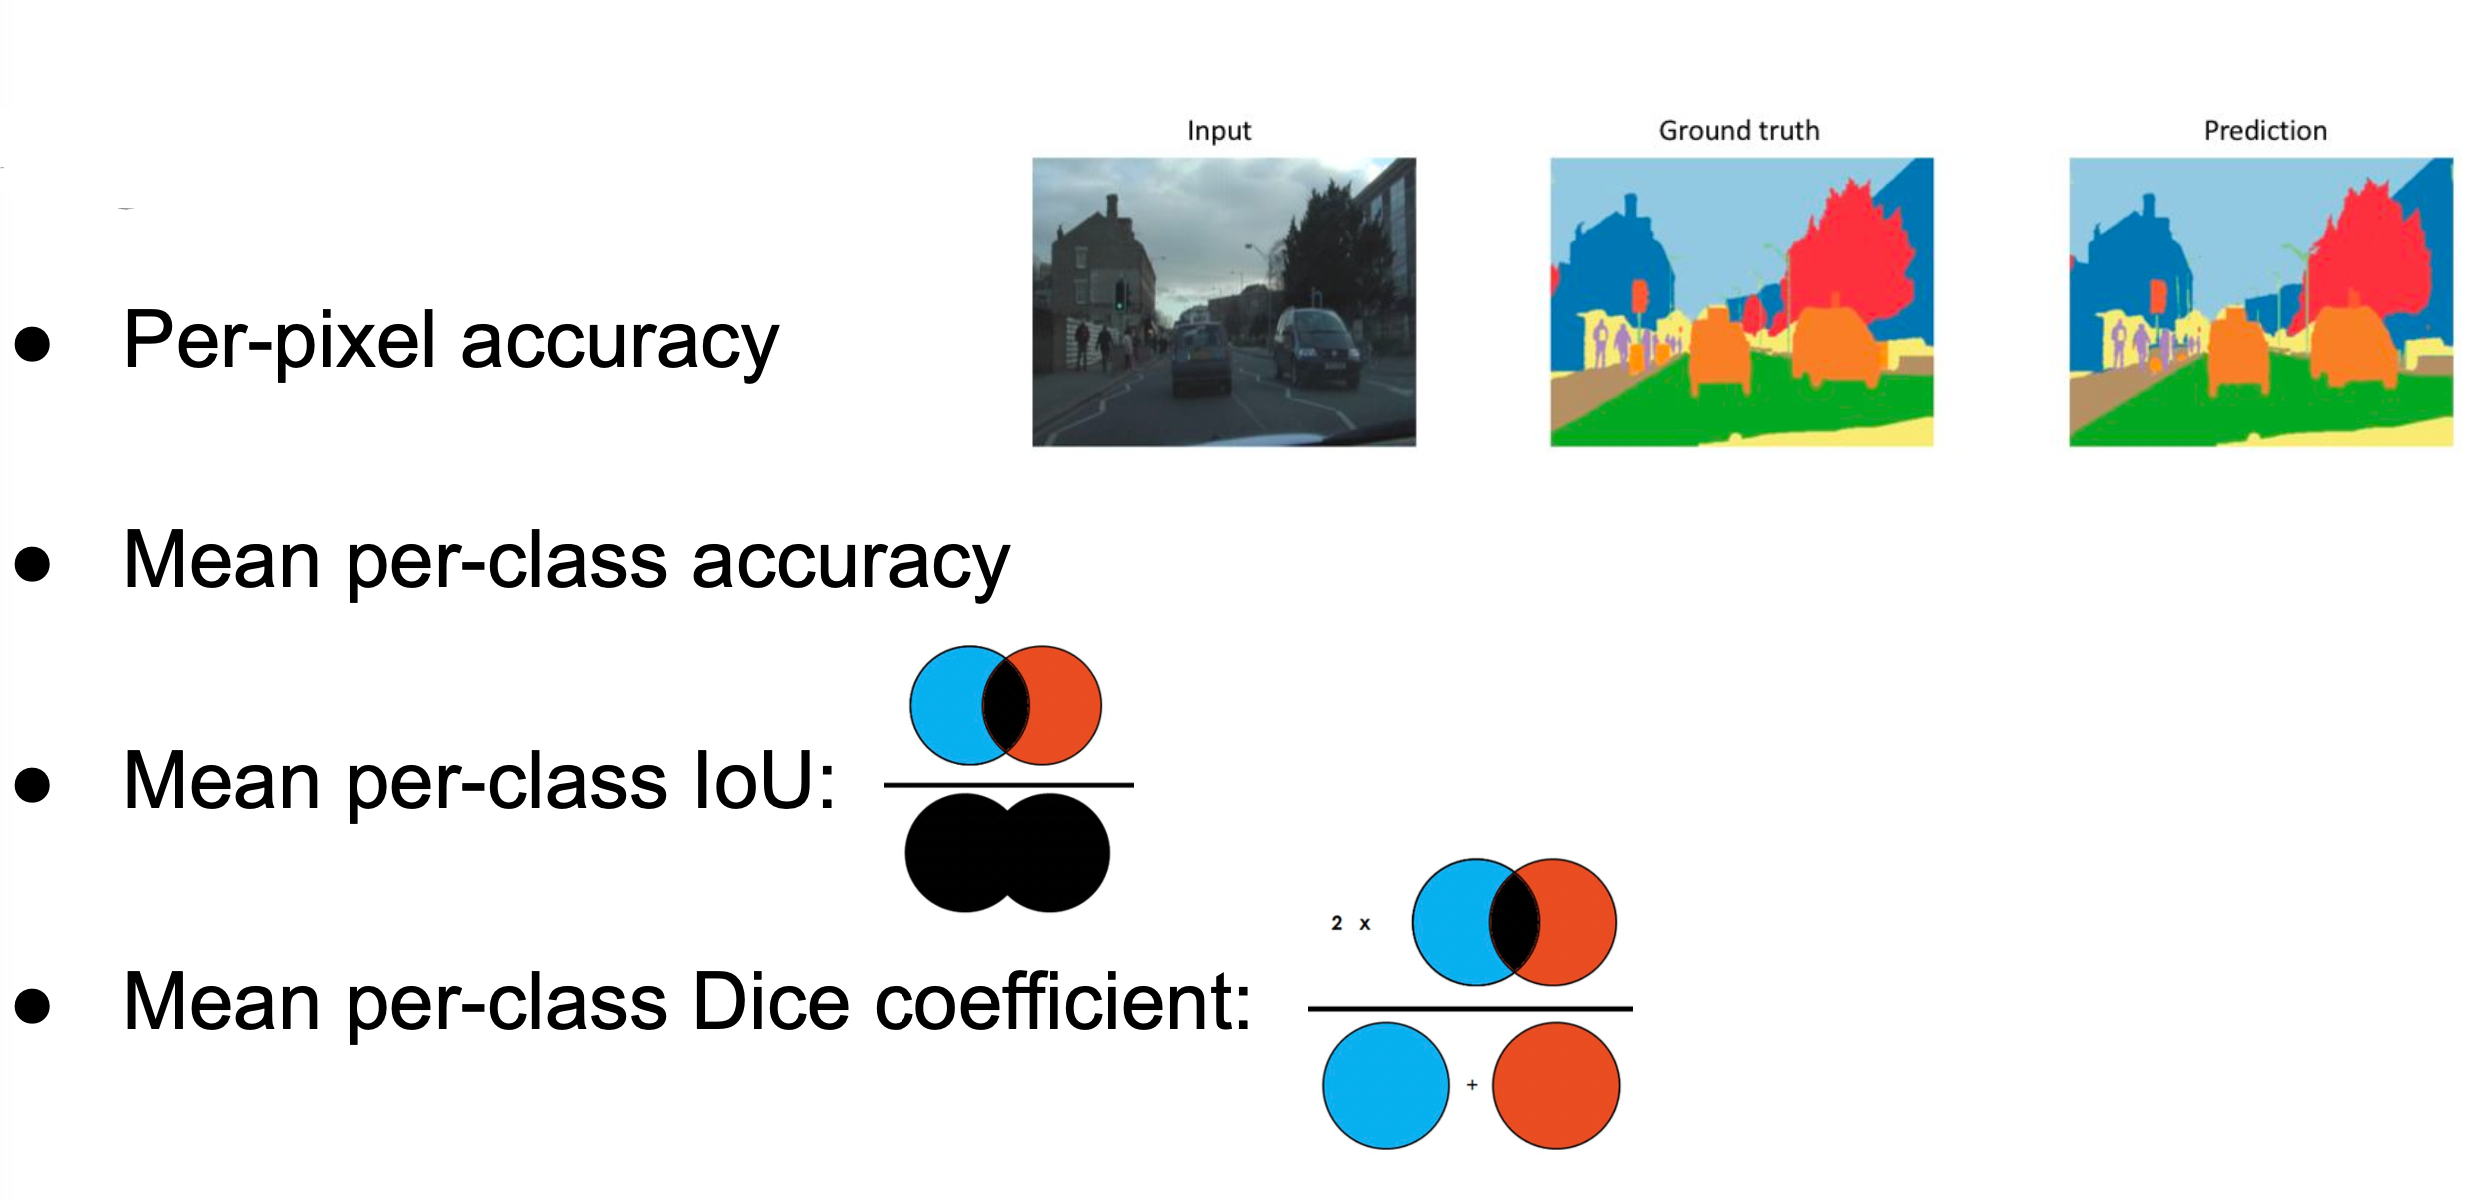
\includegraphics[width=.99\linewidth]{segm_metr.png}
	\end{center}
\end{frame}


\begin{frame}{Сегментация}
	\begin{center}
		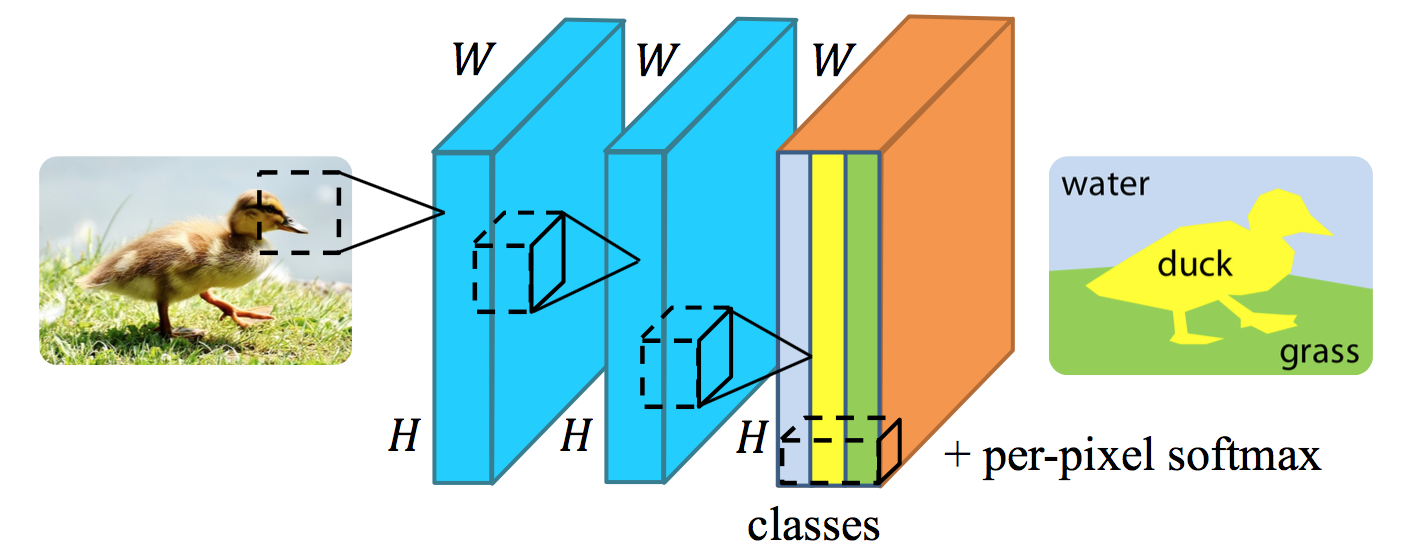
\includegraphics[width=.9\linewidth]{duck_1.png}
		%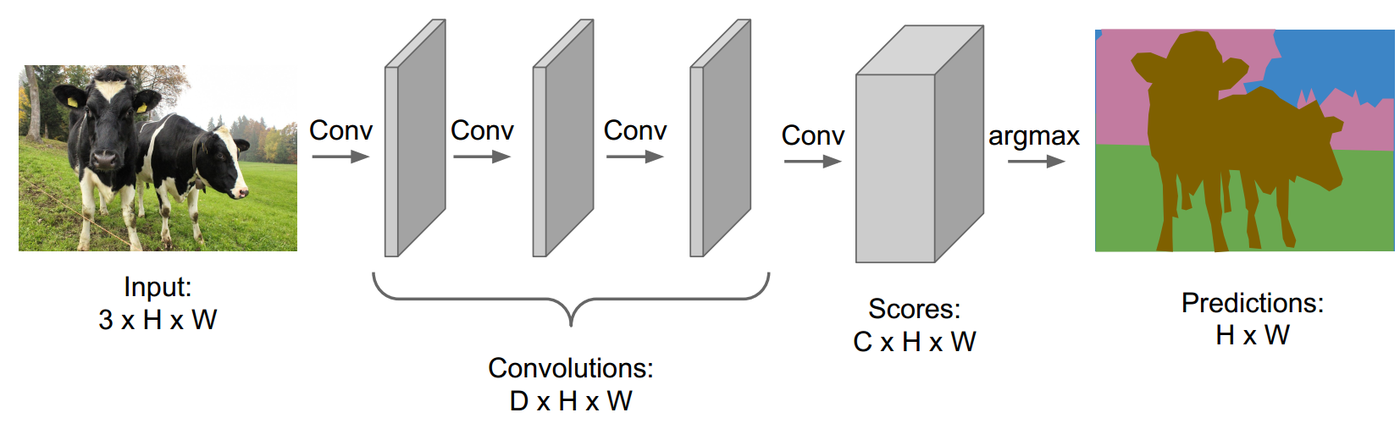
\includegraphics[width=.9\linewidth]{conv_seg.png}
	\end{center}
	\begin{itemize}
		\item Нам нужно научиться классифицировать каждый пиксель
		\item Куча свёрток и попиксельный softmax без пулинга (наивный подход)
	\end{itemize}
\end{frame}


\begin{frame}{Сегментация}
	\begin{center}
		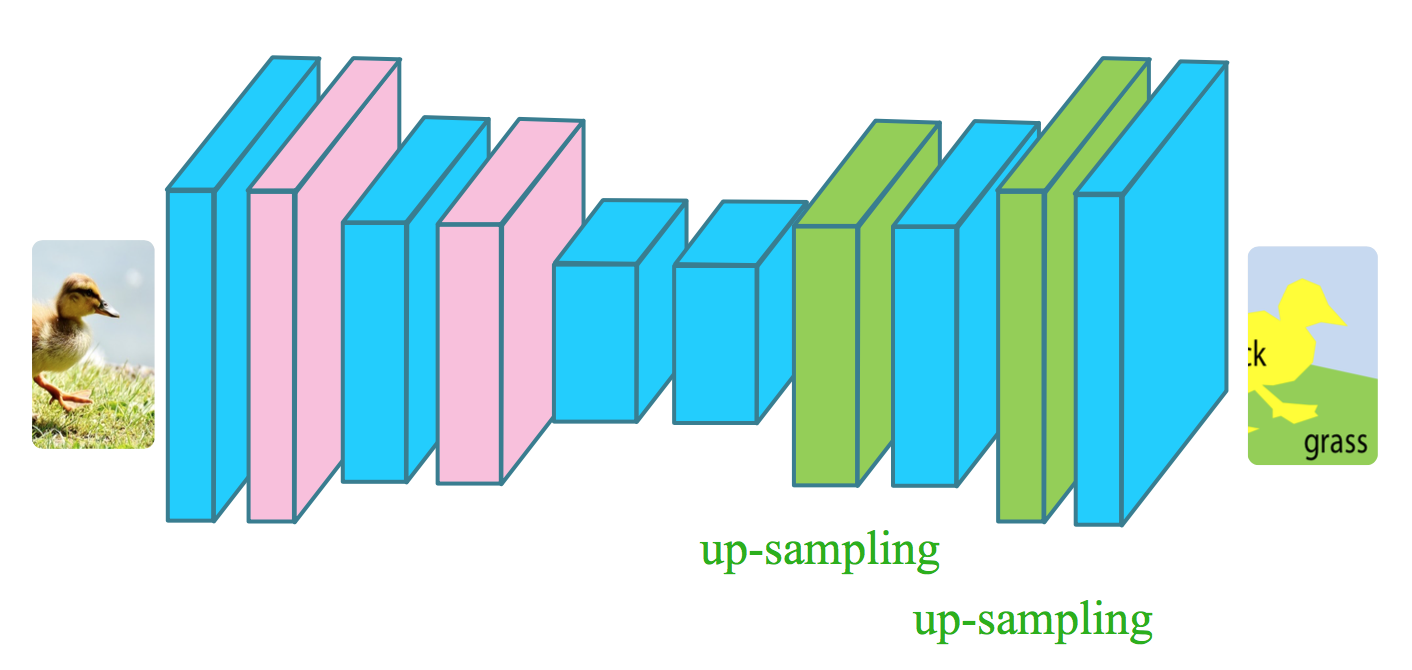
\includegraphics[width=.8\linewidth]{duck_2.png}
		%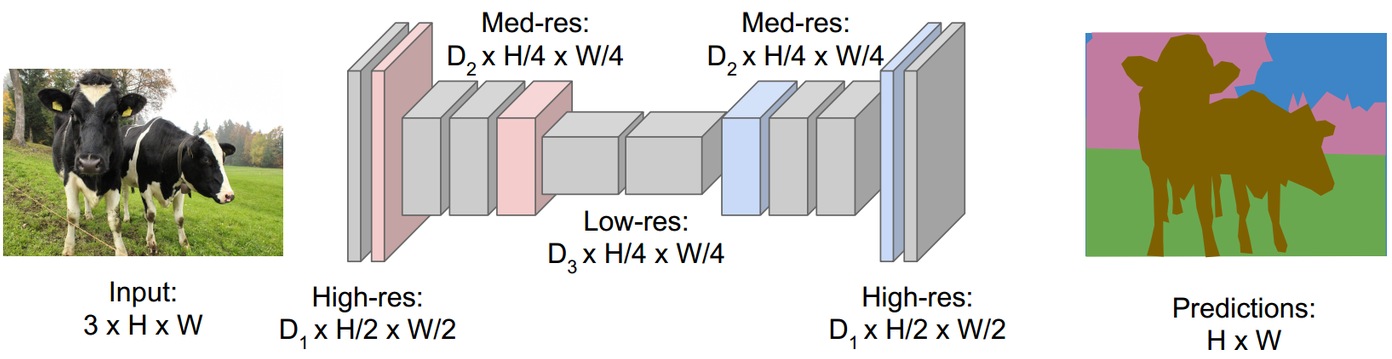
\includegraphics[width=.8\linewidth]{segm_down.png}
	\end{center}
	\begin{itemize}
		\item Если захотим добавить пулинг, придётся делать анпулинг
	\end{itemize}
\end{frame}


\begin{frame}{Nearest neighbor unpooling}
	\begin{center}
		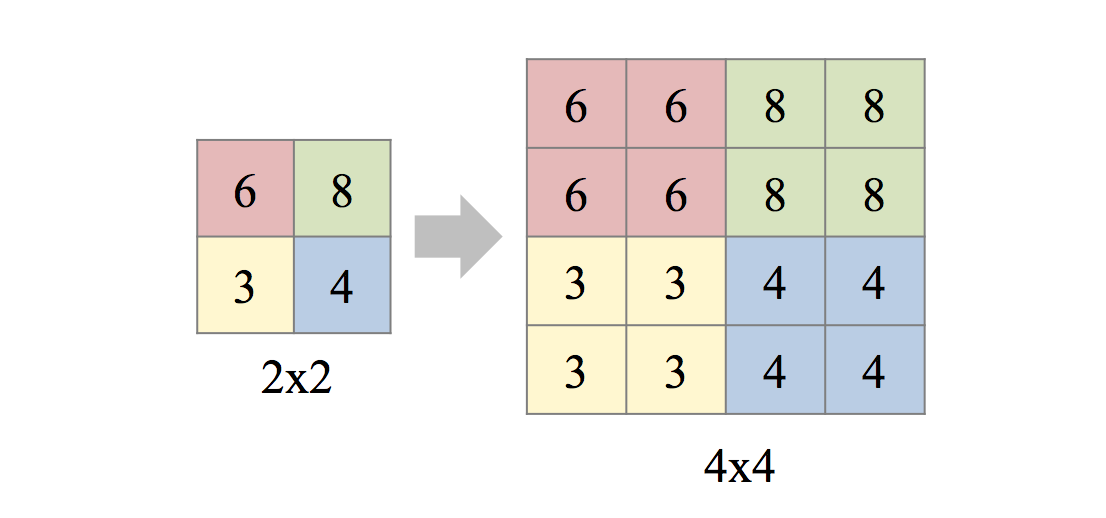
\includegraphics[width=.9\linewidth]{nnun.png}
	\end{center}
\end{frame}


\begin{frame}{Max unpooling}
	\begin{center}
		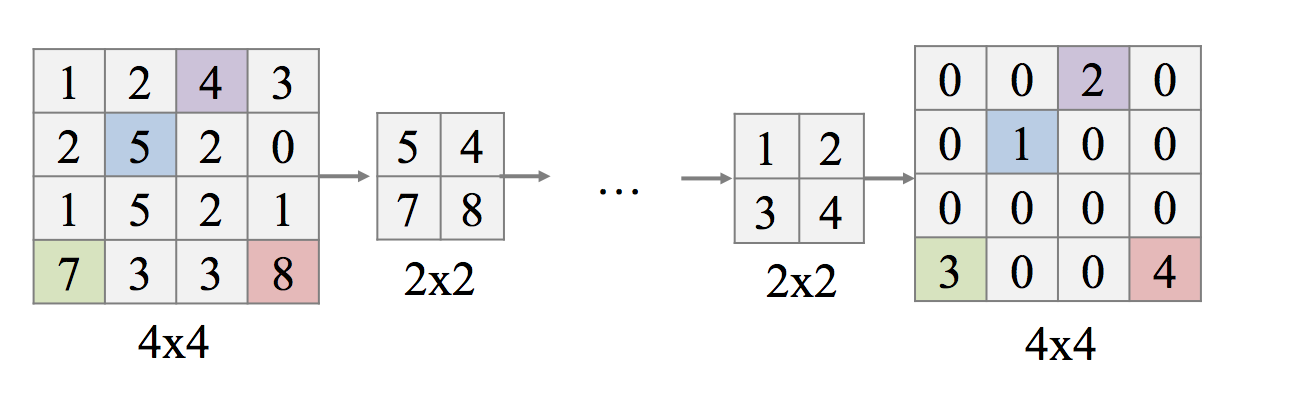
\includegraphics[width=.9\linewidth]{maxun.png}
	\end{center}
\end{frame}


\begin{frame}{Learnable unpooling: Transpose convolution}
	\begin{center}
		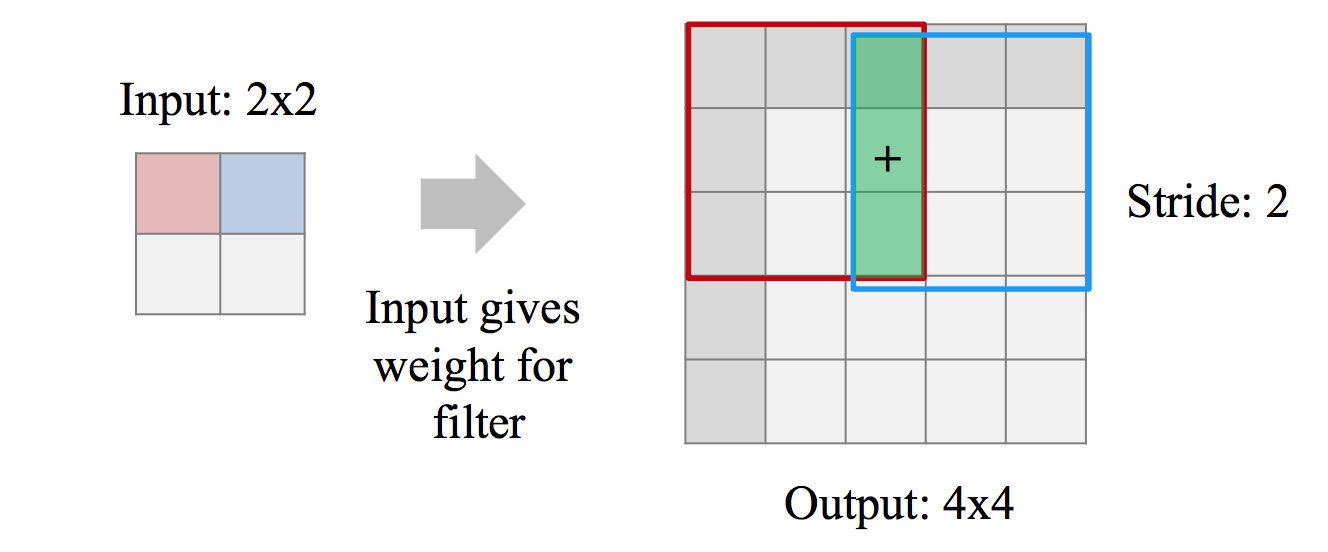
\includegraphics[width=.7\linewidth]{leun.png}
	\end{center}
	\begin{itemize}
		\item Каждую клетку надо распаковать в $4$ клетки $\Rightarrow$ свёртка $3 \times 3$ со сдвигом $2$
	\end{itemize}
\end{frame}


\begin{frame}{Пример:}
	\begin{center}
		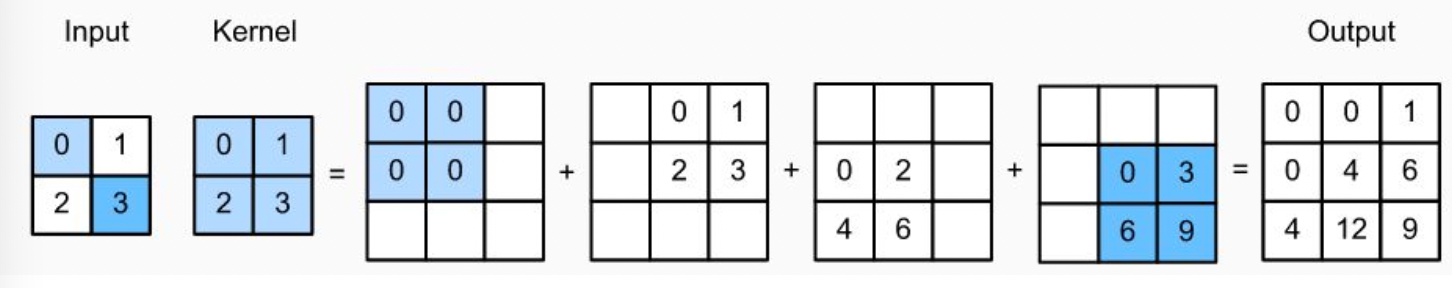
\includegraphics[width=.99\linewidth]{unpooling_ex2.png}
	\end{center}
\end{frame}


\begin{frame}{Fully-convolution net}
	\begin{center}
		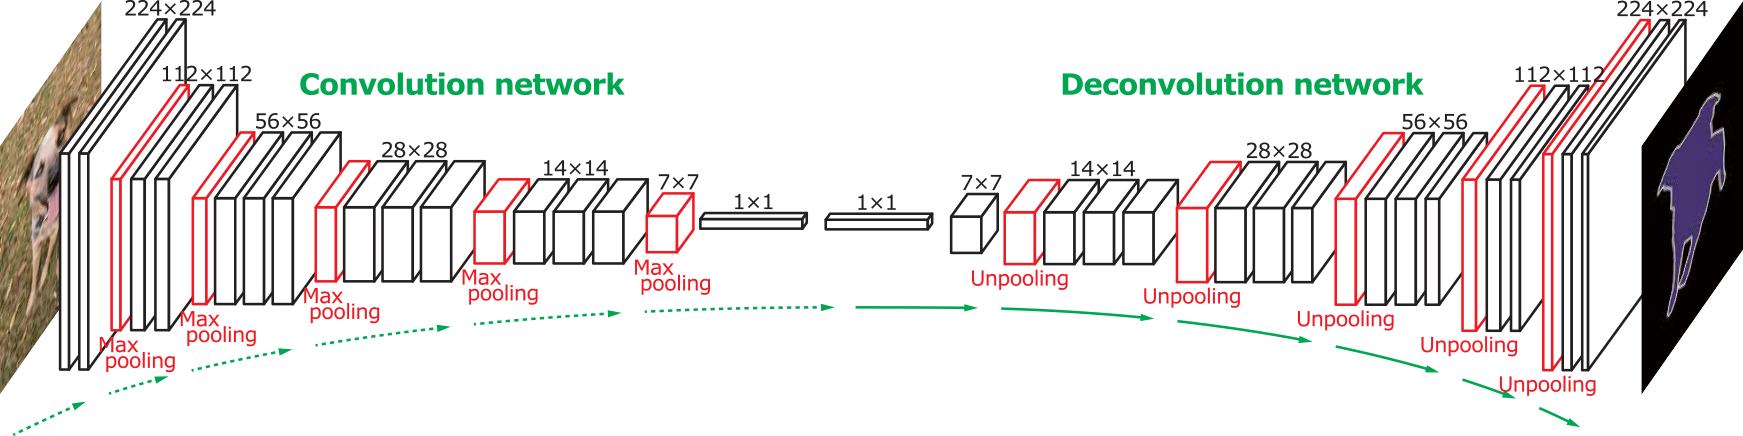
\includegraphics[width=.8\linewidth]{fully_net.png}
	\end{center}
	\begin{itemize}
		\item Cвернули в скрытое представление, развернули, спрогнозировали
	\end{itemize}
\end{frame}


\begin{frame}{ U-net (2015)}
	\begin{columns}[T] % align columns
		\begin{column}{.38\textwidth}
			\begin{wideitemize}	
				\item Можно добавить связи между слоями, отражающими одинаковую абстракцию, это должно улучшить модель
				\item По-прежнему используем транспонированную свёртку
			\end{wideitemize}
		\end{column}%
		\hfill%
		\begin{column}{.62\textwidth}
			\begin{center}
				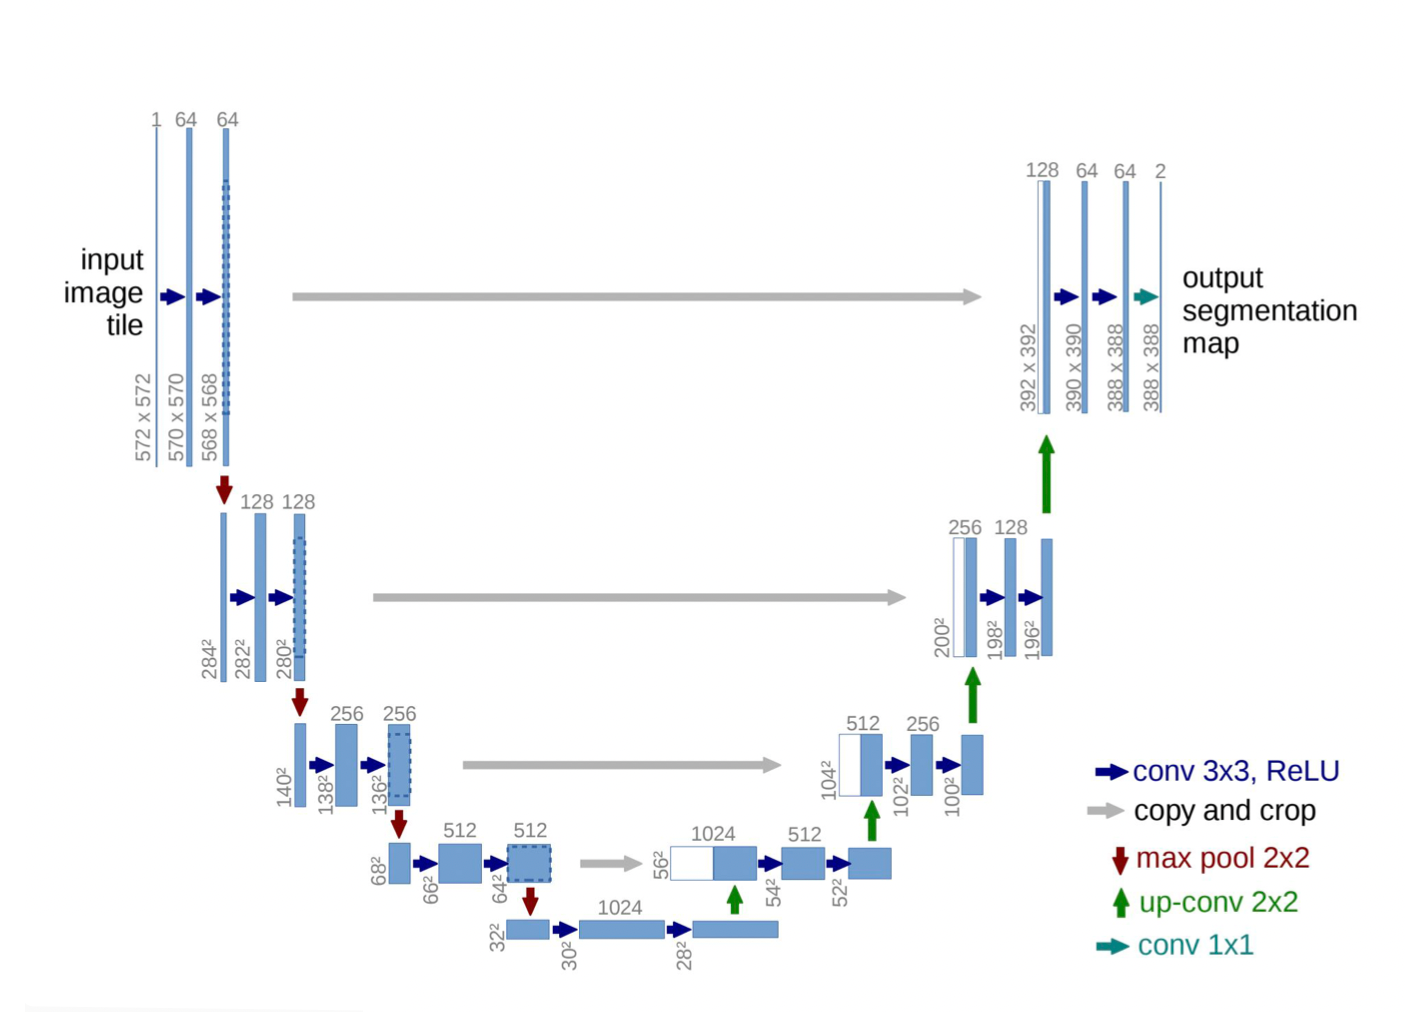
\includegraphics[width=.99\linewidth]{unet.png}
			\end{center} 
		\end{column}%
	\end{columns}
	\vfill
	\footnotesize
	{\color{blue} \url{https://arxiv.org/abs/1505.04597}} 
\end{frame}


\begin{transitionframe}
	\begin{center}
		\Huge  Векторные представления картинок (эмбеддинги)
	\end{center}
\end{transitionframe}


\begin{frame}{Представления с последних слоёв}
	\begin{wideitemize}
		\item  Выходы с последних слоёв свёрточных нейросетей являются хорошими признаковыми описаниями изображений
		\item Такие векторные представления называют \alert{эмбеддингами (embeddings)}
		\item У эмбеддингов нет чёткой интерпретации, цифры в них говорят о наличии каких-то паттернов, на которые настроилась нейросетка
		\item Эмбеддинги картинок оказываются полезными во многих задачах 
	\end{wideitemize}
\end{frame}


\begin{frame}{TSNE для CIFAR-10 (предпоследний слой простой свёрточной сетки)}
	\begin{center}
		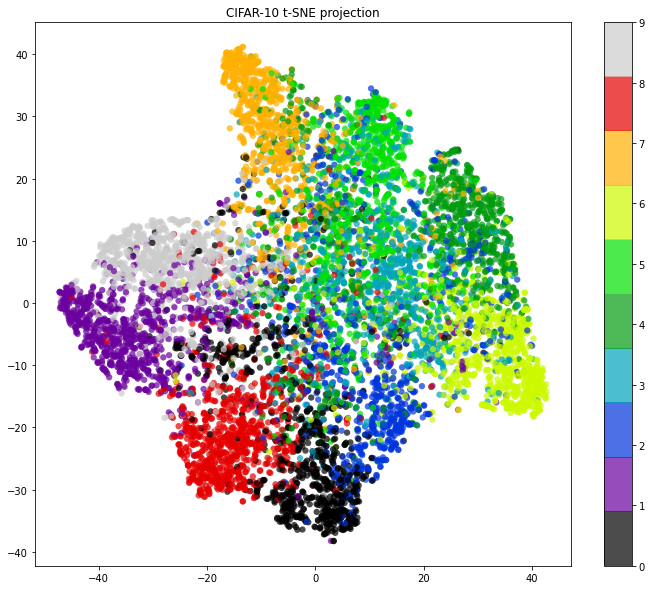
\includegraphics[width=.5\linewidth]{tsne_conv.png}
	\end{center}
\end{frame}


\begin{frame}{Представления изображений}
	\begin{center}
		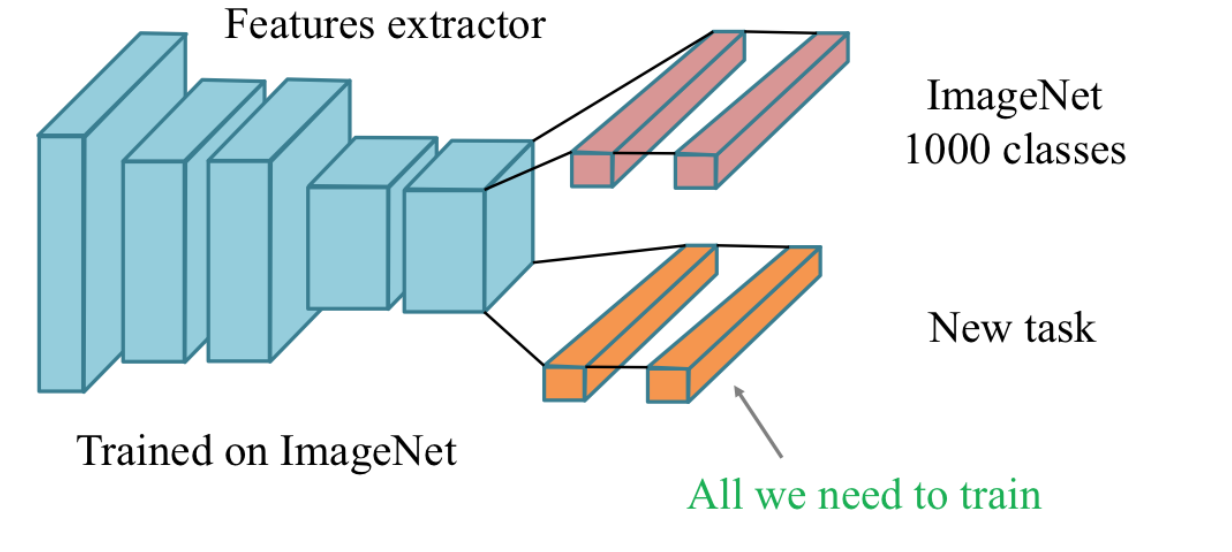
\includegraphics[width=.8\linewidth]{transfer_learning2.png}
	\end{center}
\end{frame}


\begin{frame}{Дообучение (Transfer learning)}
	\begin{wideitemize}
		\item Если данных совсем мало
		\item Берём модель из другой задачи
		\item Заменяем последний слой на слой с нужным числом выходов
		\item Обучаем только его
		\item По сути, это обучение линейной модели на эмбединге картинки
		\item Иногда приходится дообучать часть экстрактора эмбедингов
	\end{wideitemize}
\end{frame}


\begin{frame}{Представления изображений}
	\begin{wideitemize}
		\item  Выход предпоследнего полносвязного слоя — хорошее
		представления картинки
		\item  Но для его обучения нужны изображения с разметкой
		\item  Может, получится строить такие представления и без разметки?	
		\item  Ведь для текстов получилось, мы собрали w2v
		\item  Нужна какая-то фейковая задача
	\end{wideitemize}
\end{frame}


\begin{transitionframe}
	\begin{center}
		\Huge  Автокодировщики
	\end{center}
\end{transitionframe}


\begin{frame}{Автокодировщики}
	\begin{center}
		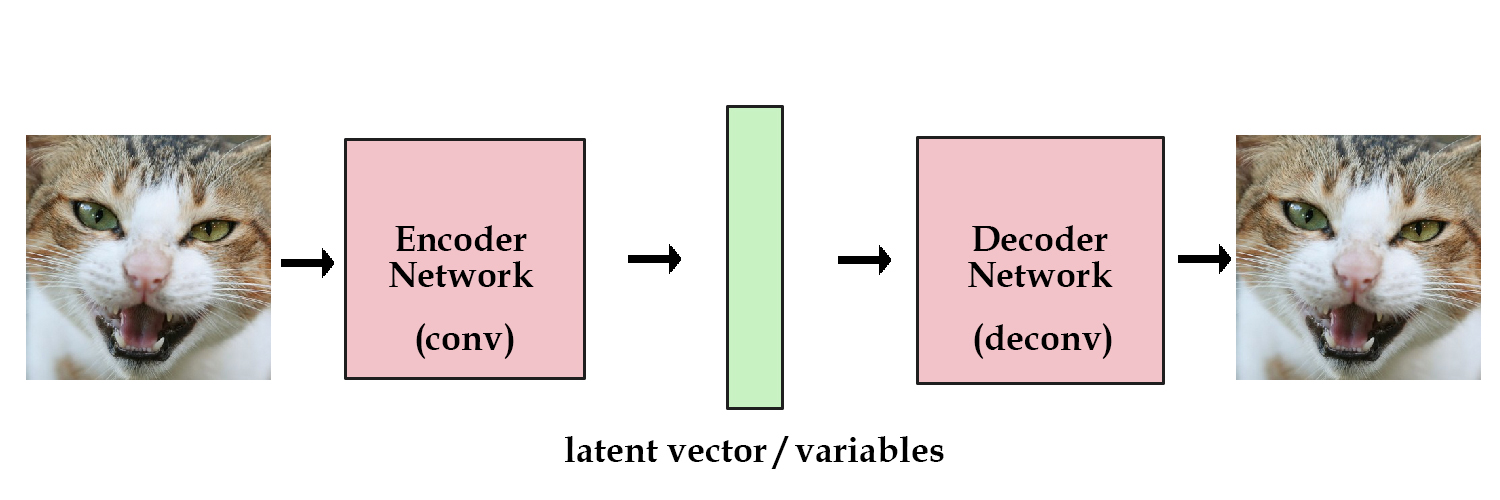
\includegraphics[width=.9\linewidth]{autoencoder.png}
	\end{center}
\end{frame}


\begin{frame}{Автокодировщики}
	\begin{center}
		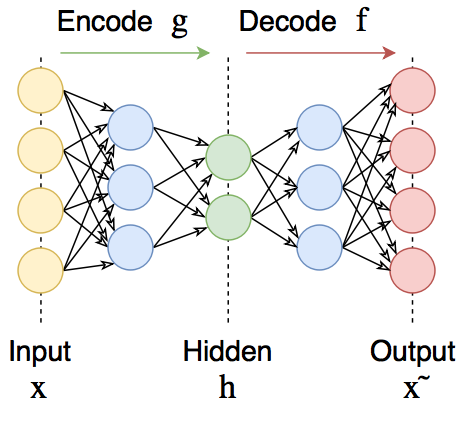
\includegraphics[width=.42\linewidth]{auto.png}
	\end{center} \pause
	\[
	\frac{1}{n} \sum_{i=1}^n L(x_i, f(g(x_i))) \to \min 
	\]
\end{frame}


\begin{frame}{Пример сжатия}
	\begin{center}
		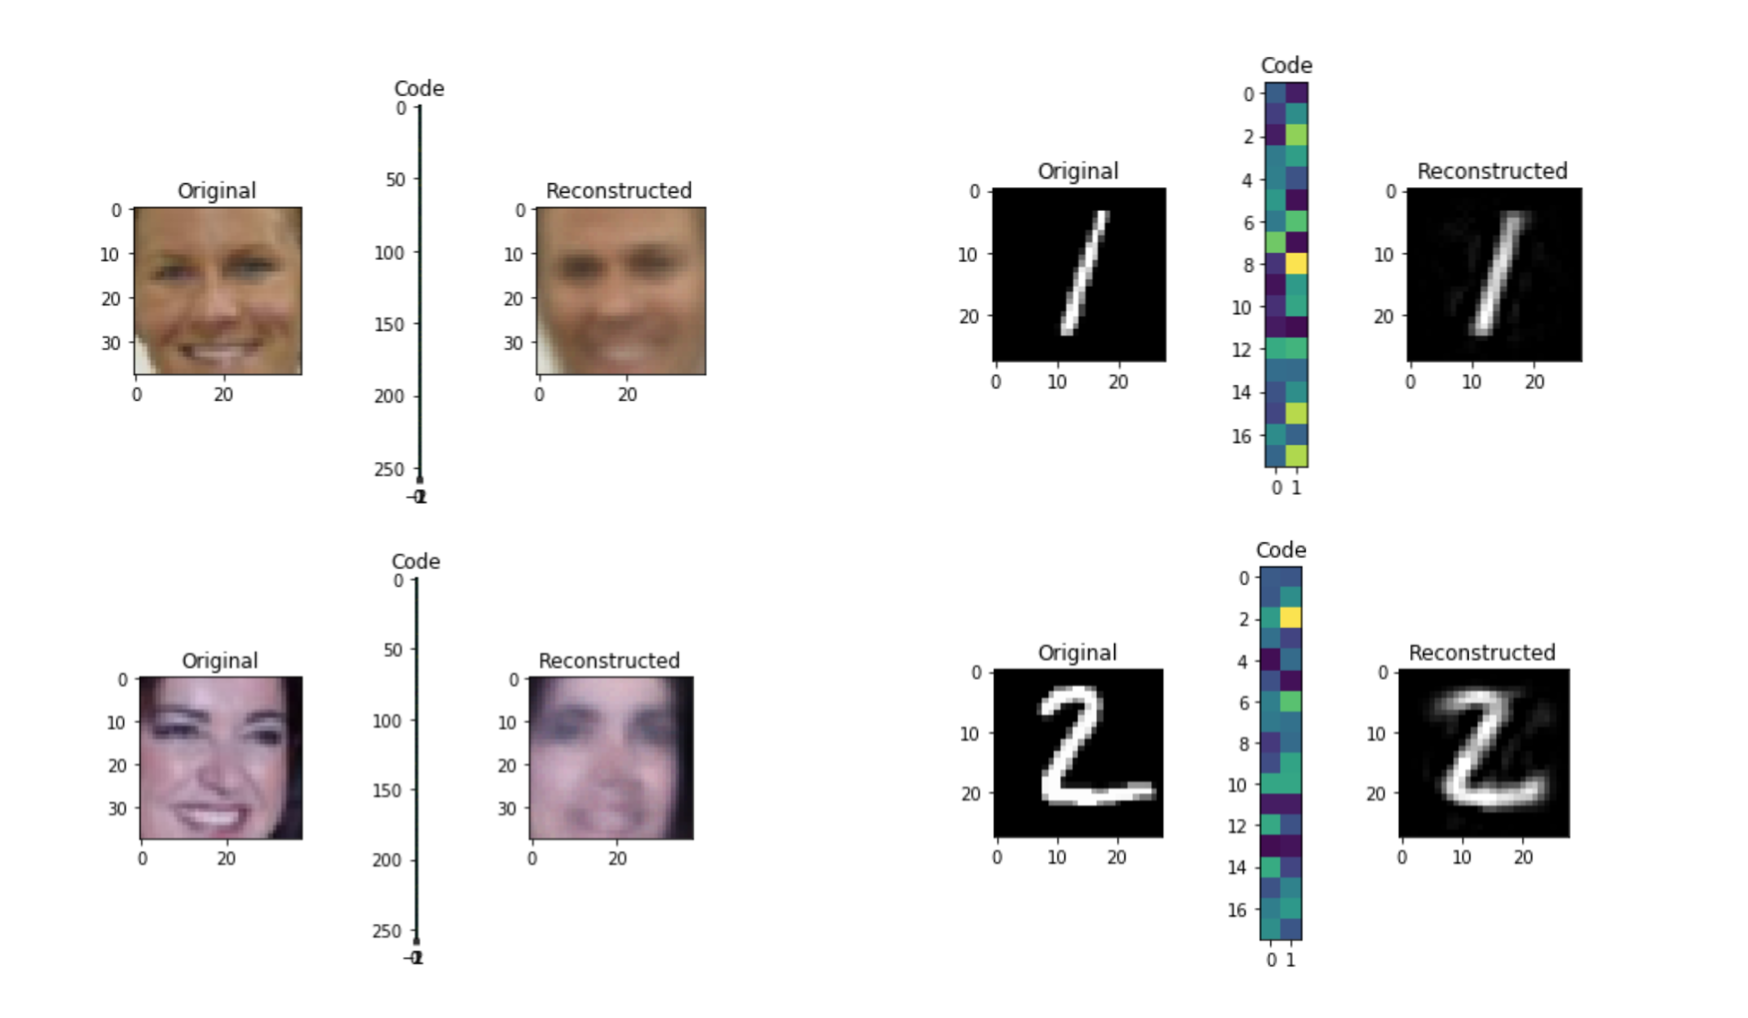
\includegraphics[width=.8\linewidth]{ato_enc.png}
	\end{center}
\end{frame}

\begin{frame}{Зачем это всё?}
	\begin{wideitemize}
		\item  Сжатие данных (нелинейных аналог PCA)
		\item  Очистка картинки от шума
		\item  Поиск похожих изображений
		\item  Трансформация изображений
		\item  Генерация изображений
	\end{wideitemize}
\end{frame}


\begin{frame}{Автокодировщики}
	\begin{wideitemize}
		\item  Понижают размерность, исходная картинка восстанавливается с потерями
		\item  Основная ценность — эмбединг из булочного горлышка, хочется чтобы он получился максимально качественным
		\item  Наша архитектура сильно переобучается под выборку, для новых лиц работает хуже
		\item  Нужна регуляризация, которая позволит извлекать смысл, а не восстанавливать пиксели в точности (фон тоже запоминается)
	\end{wideitemize}
\end{frame}


\begin{frame}{Denoising autoencoder}
	\begin{center}
		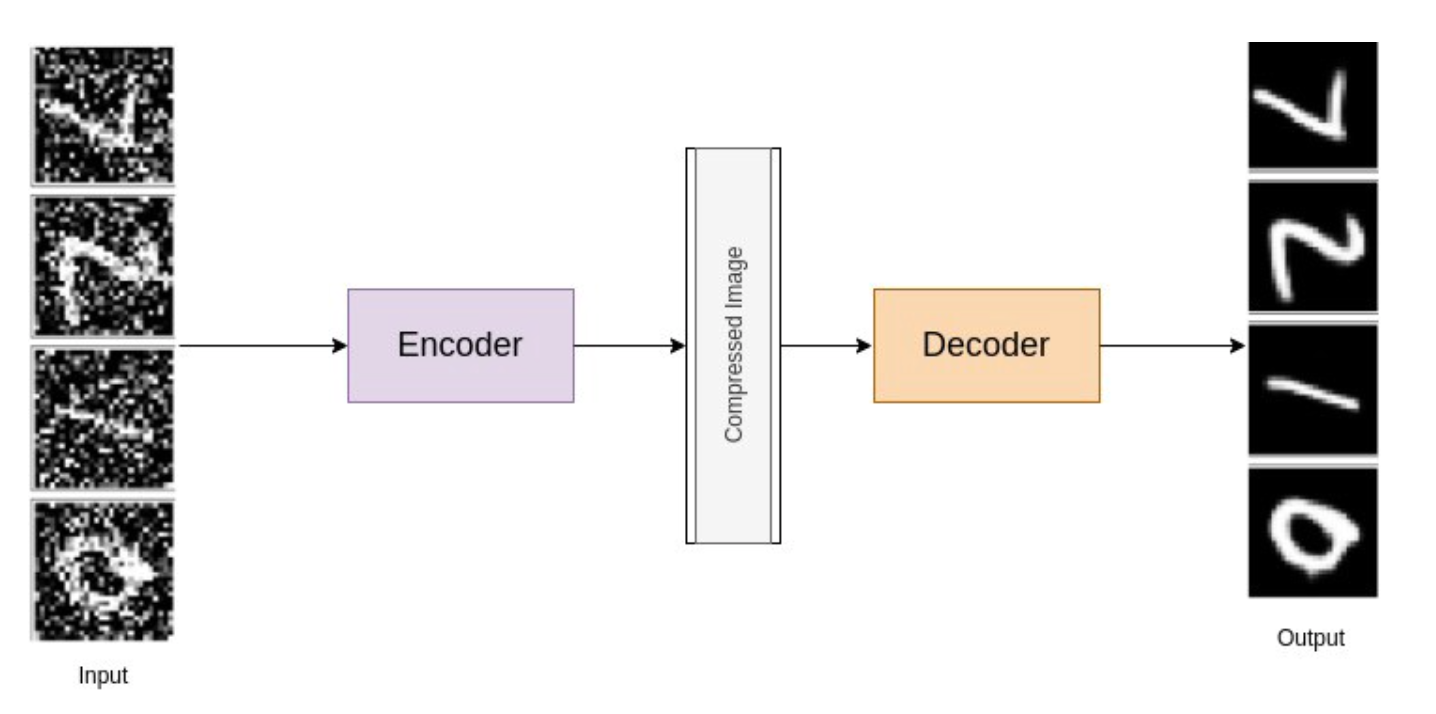
\includegraphics[width=.8\linewidth]{denoise.png}
	\end{center}
	\vfill
	\footnotesize
	{\color{blue} \url{https://medium.com/@garimanishad/reconstruct-corrupted-data-using-denoising-autoencoder-python-code-aeaff4b0958e} \newline \url{https://www.cs.toronto.edu/~larocheh/publications/icml-2008-denoising-autoencoders.pdf} } 
\end{frame}


\begin{frame}{Morphing faces}
	\begin{center}
		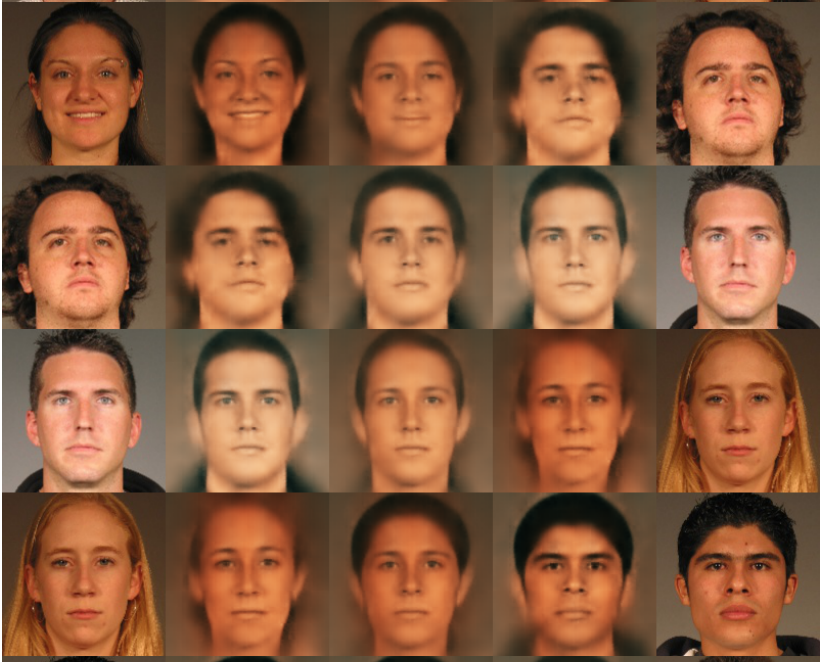
\includegraphics[width=.5\linewidth]{morth.png}
	\end{center}
	\vfill
	\footnotesize
	{\color{blue} \url{http://essay.utwente.nl/81372/1/Heuver_MA_EEMCS.pdf}  } 
\end{frame}


\begin{frame}{Morphing faces}
	\begin{center}
		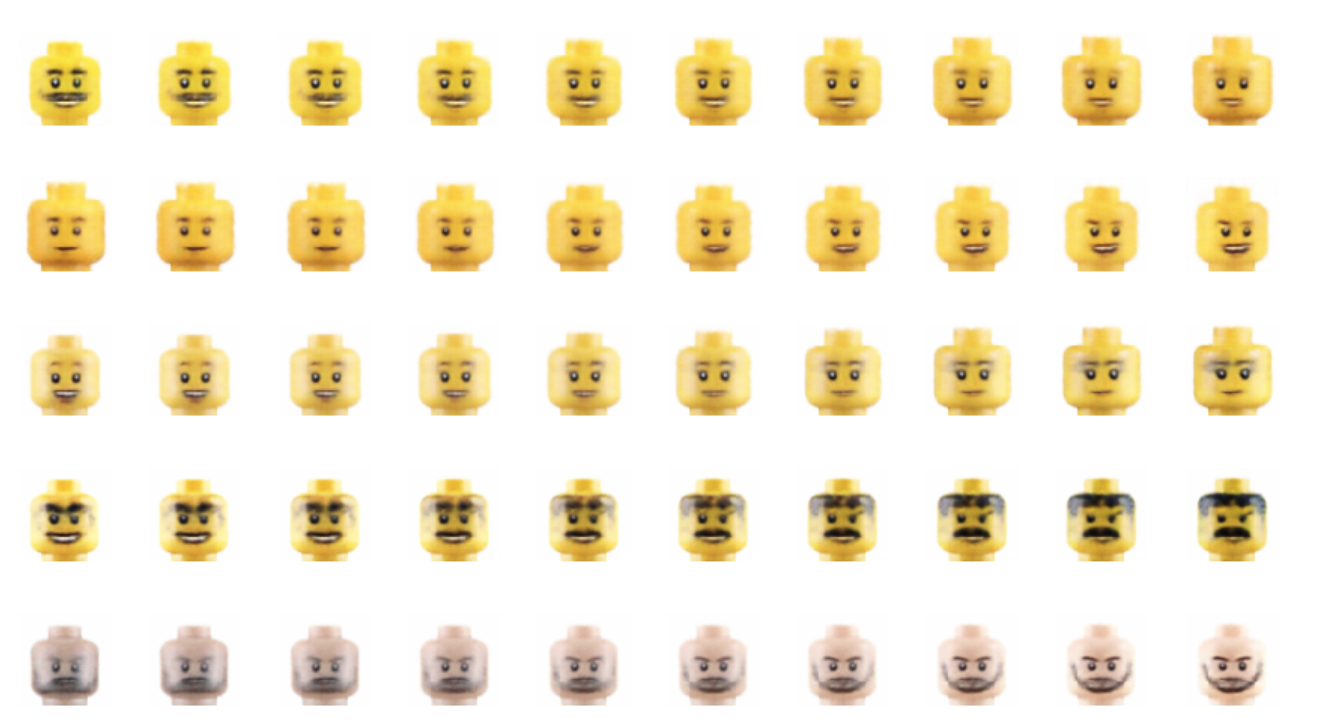
\includegraphics[width=.85\linewidth]{lego.png}
	\end{center}
	\vfill
	\footnotesize
	{\color{blue} \url{https://www.echevarria.io/blog/lego-face-vae/index.html}  } 
\end{frame}


\begin{frame}{Саморегуляция выборки}
	\begin{center}
		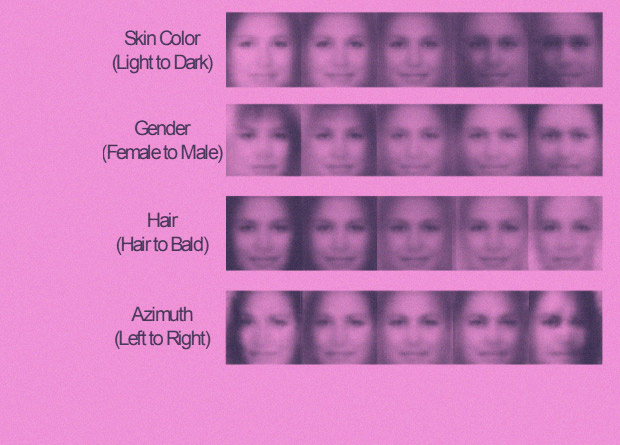
\includegraphics[width=.6\linewidth]{avtoreg.png}
	\end{center}
	\vfill
	\footnotesize
	{\color{blue} \url{https://nplus1.ru/news/2019/01/28/debiasing-faces}  } 
\end{frame}


\begin{frame}{Поиск фрода}
	\begin{center}
		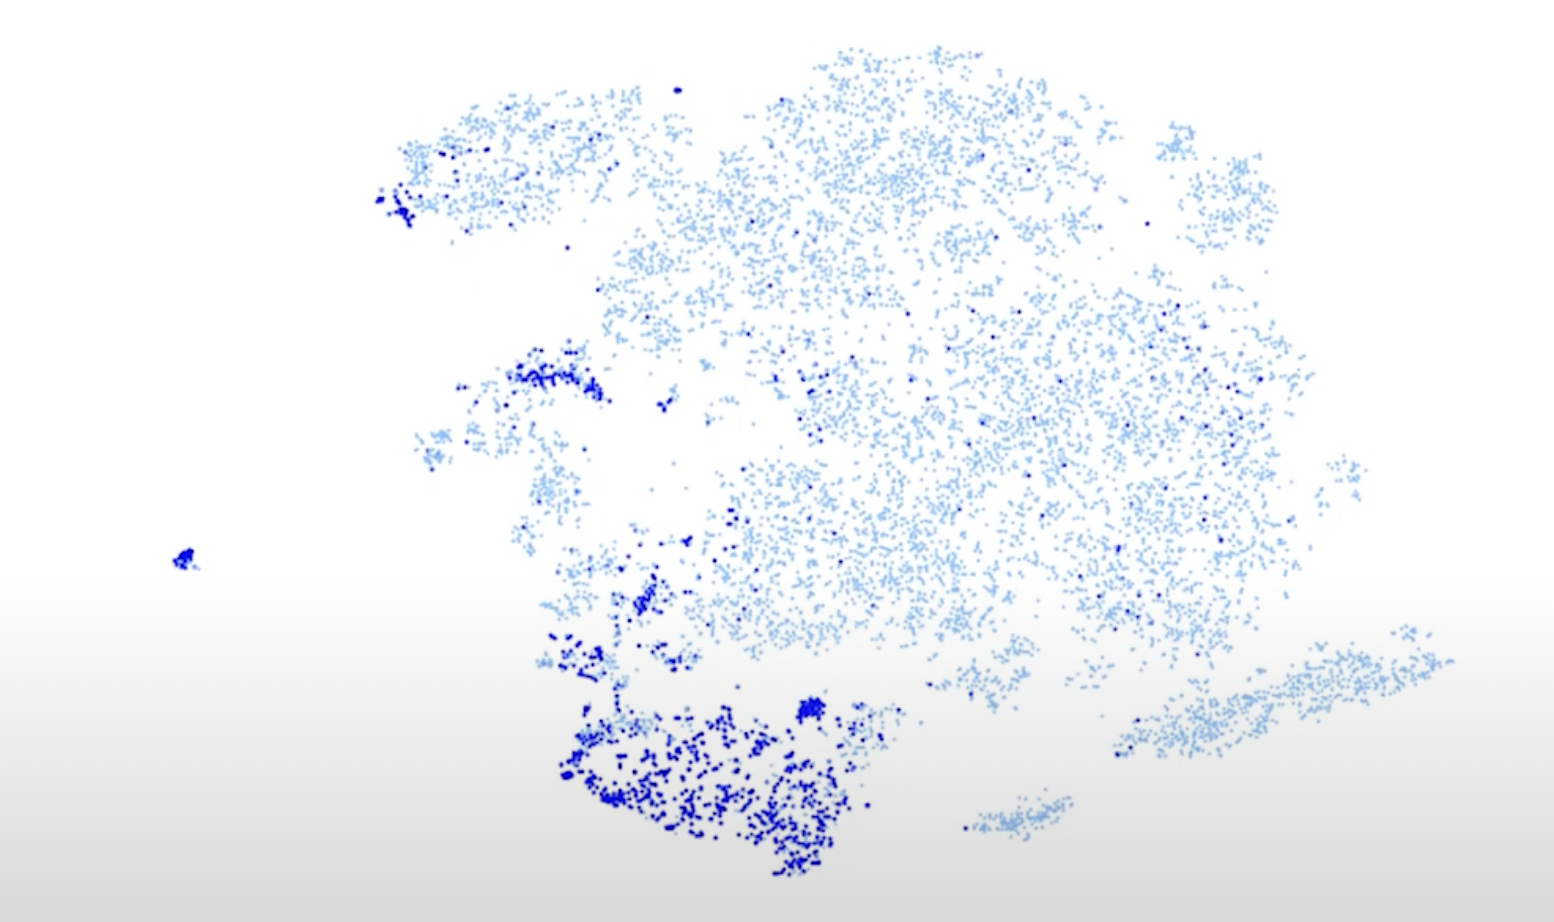
\includegraphics[width=.7\linewidth]{yandex_tsne.png}
	\end{center}
	\vfill
	\footnotesize
	Автокодировщики в антифроде Яндекса: {\color{blue} \url{https://www.youtube.com/watch?v=aBckDgtG0Zs}  } 
\end{frame}




%\begin{transitionframe}
%	\begin{center}
%		\Huge Перенос стиля 
%	\end{center}
%\end{transitionframe}
%
%
%\begin{frame}{Приложение Prisma}
%\begin{center}
%	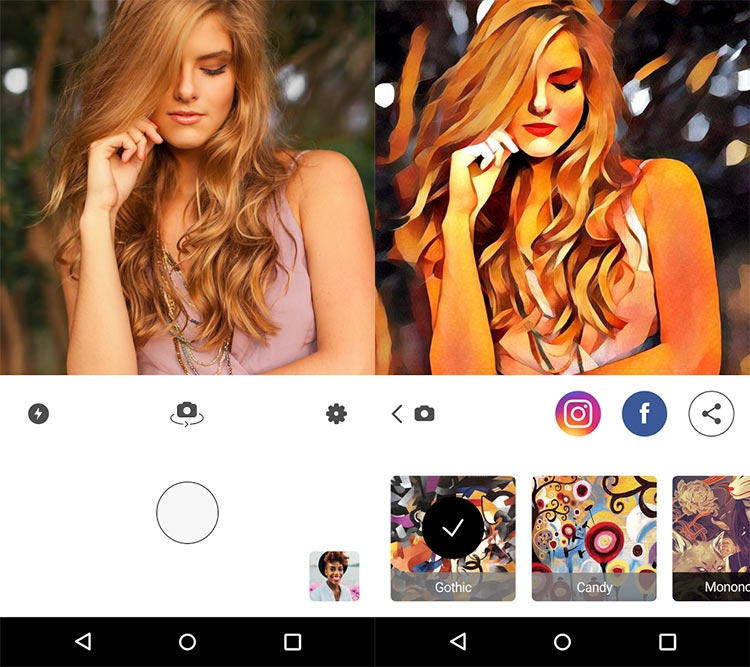
\includegraphics[width=.5\linewidth]{prisma.jpg}
%\end{center}
%\end{frame}
%
%
%\begin{frame}{Перенос стиля}
%\begin{center}
%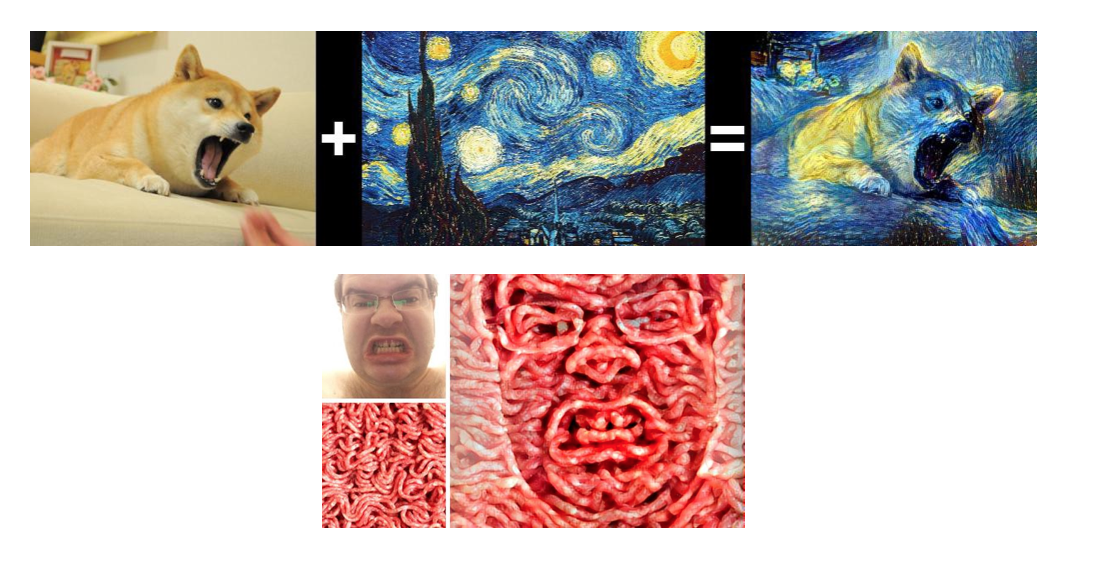
\includegraphics[width=.95\linewidth]{transfer_style.png}
%\end{center}
%\end{frame}
%
%
%\begin{frame}{Перенос стиля}
%\begin{center}
%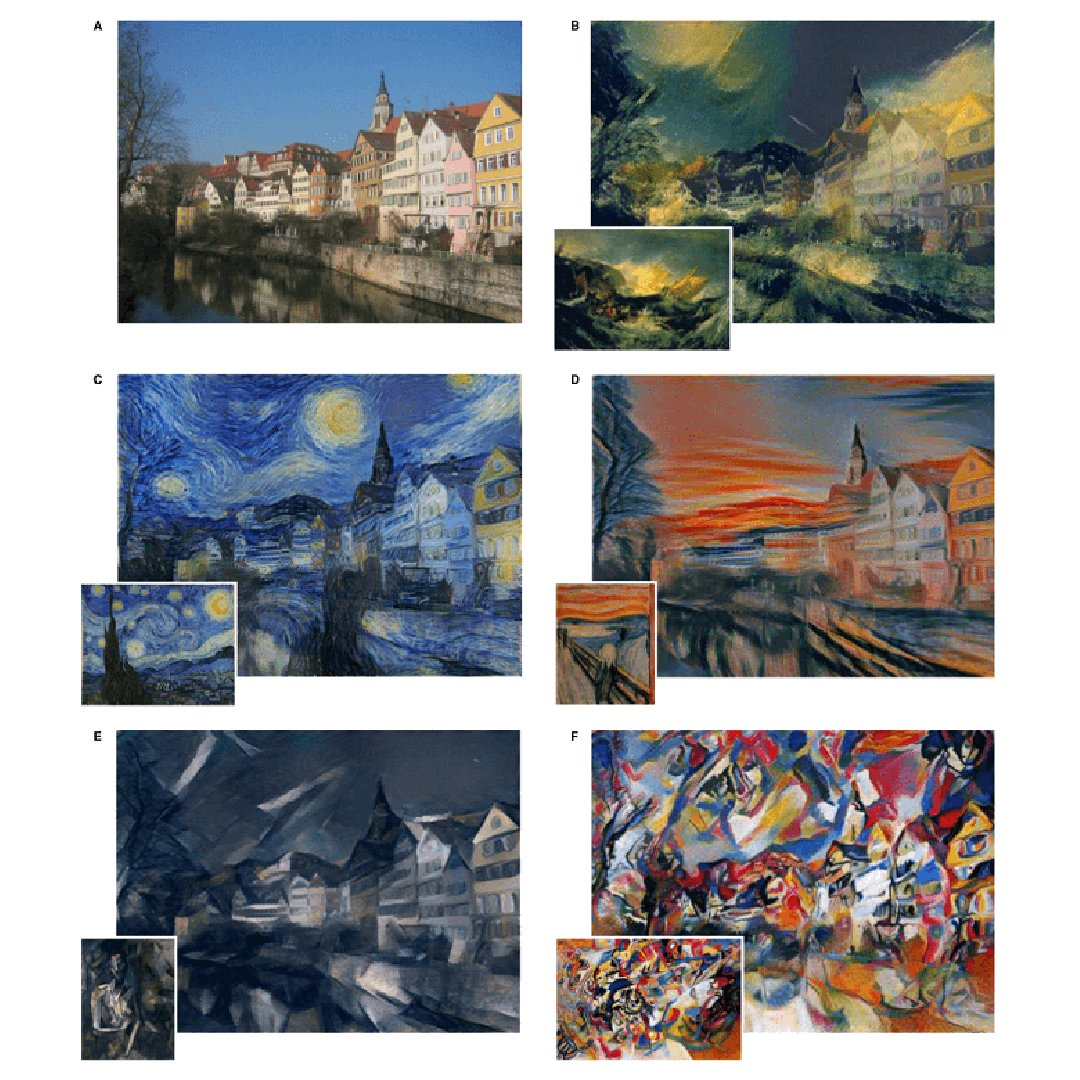
\includegraphics[width=.5\linewidth]{transfer_style_2.jpg}
%\end{center}
%\end{frame}
%
%
%\begin{frame}
%\begin{center}
%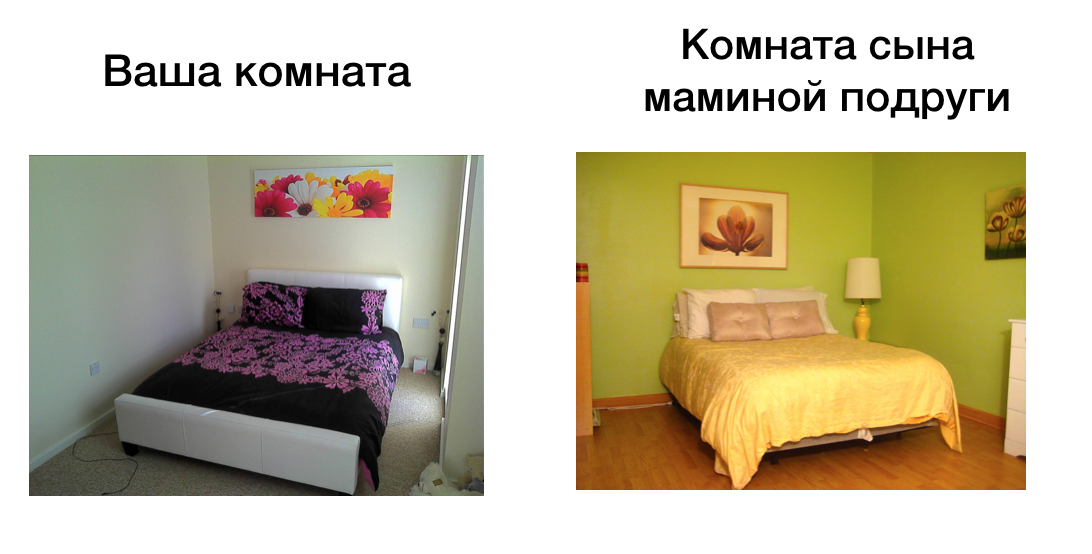
\includegraphics[width=.9\linewidth]{mom_room_1.png}
%\end{center}
%
%\vfill
%\footnotesize
%{\color{blue} \url{https://habr.com/ru/post/402665/}} \newline 
%{\color{blue} \url{https://github.com/LouieYang/deep-photo-styletransfer-tf}} 
%\end{frame}
%
%
%\begin{frame}
%\begin{center}
%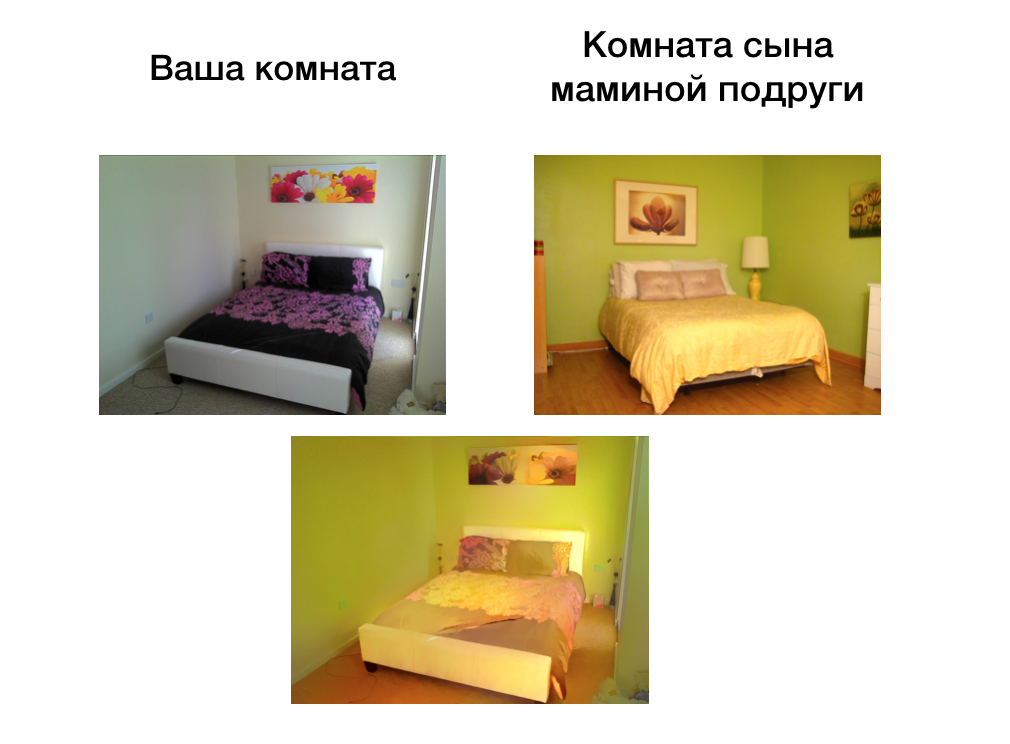
\includegraphics[width=.78\linewidth]{mom_room_2.png}
%\end{center}
%\end{frame}
%
%
%\begin{frame}
%\begin{center}
%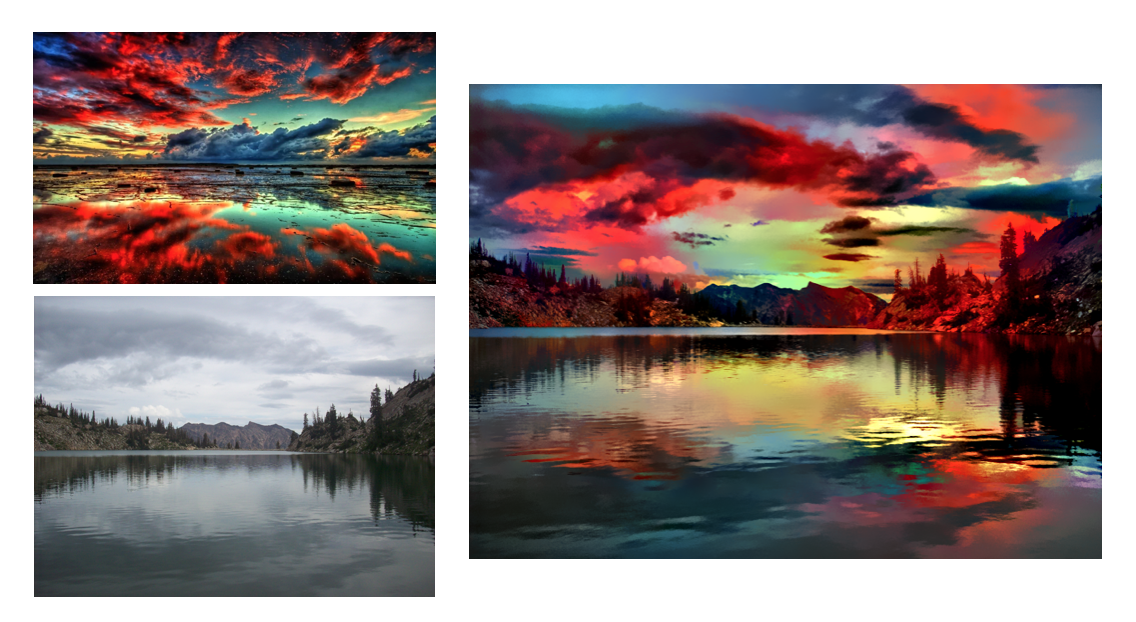
\includegraphics[width=.9\linewidth]{mom_room_3.png}
%\end{center}
%\end{frame}
%
%
%\begin{frame}
%\begin{center}
%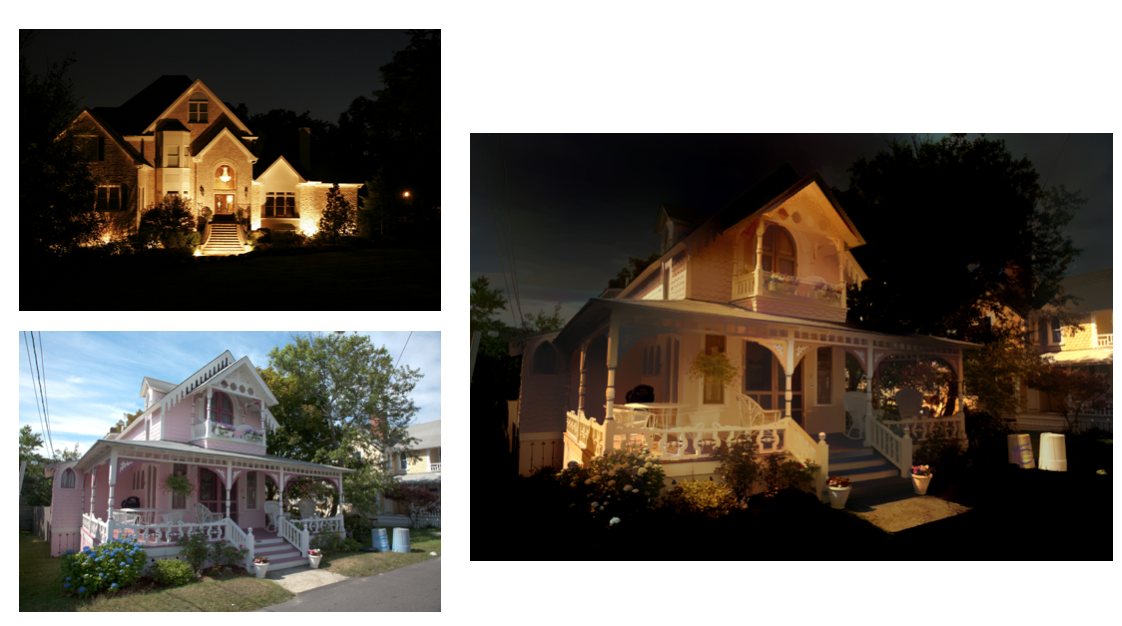
\includegraphics[width=.9\linewidth]{mom_room_4.png}
%\end{center}
%\end{frame}
%
%
%\begin{frame}{Опять этот слайд!}
%\begin{center}
%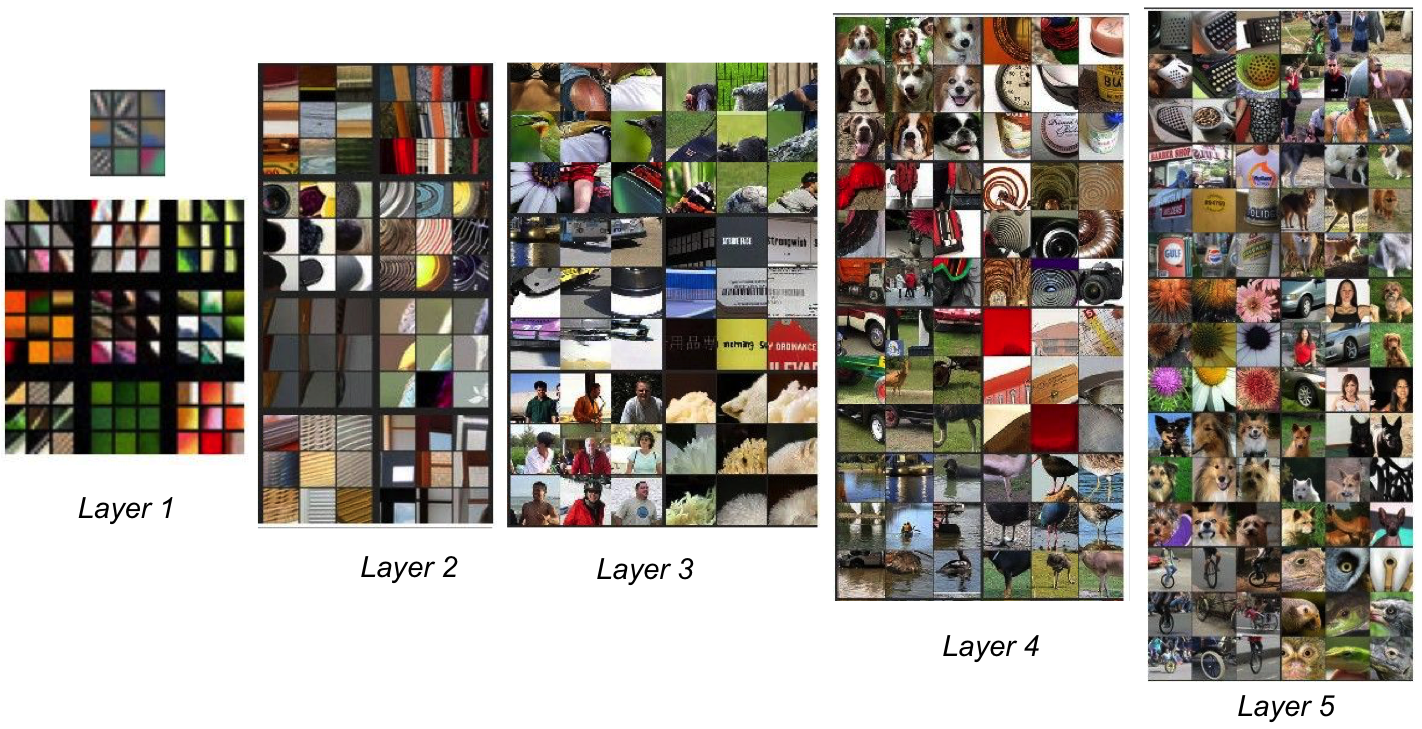
\includegraphics[width=.85\linewidth]{cnn_vis.png}
%\end{center}
%
%Есть несколько способов заглянуть внутрь свёрточной сетки, мы сейчас посмотрим на один из них
%\end{frame}
%
%\begin{frame}
%\begin{center}
%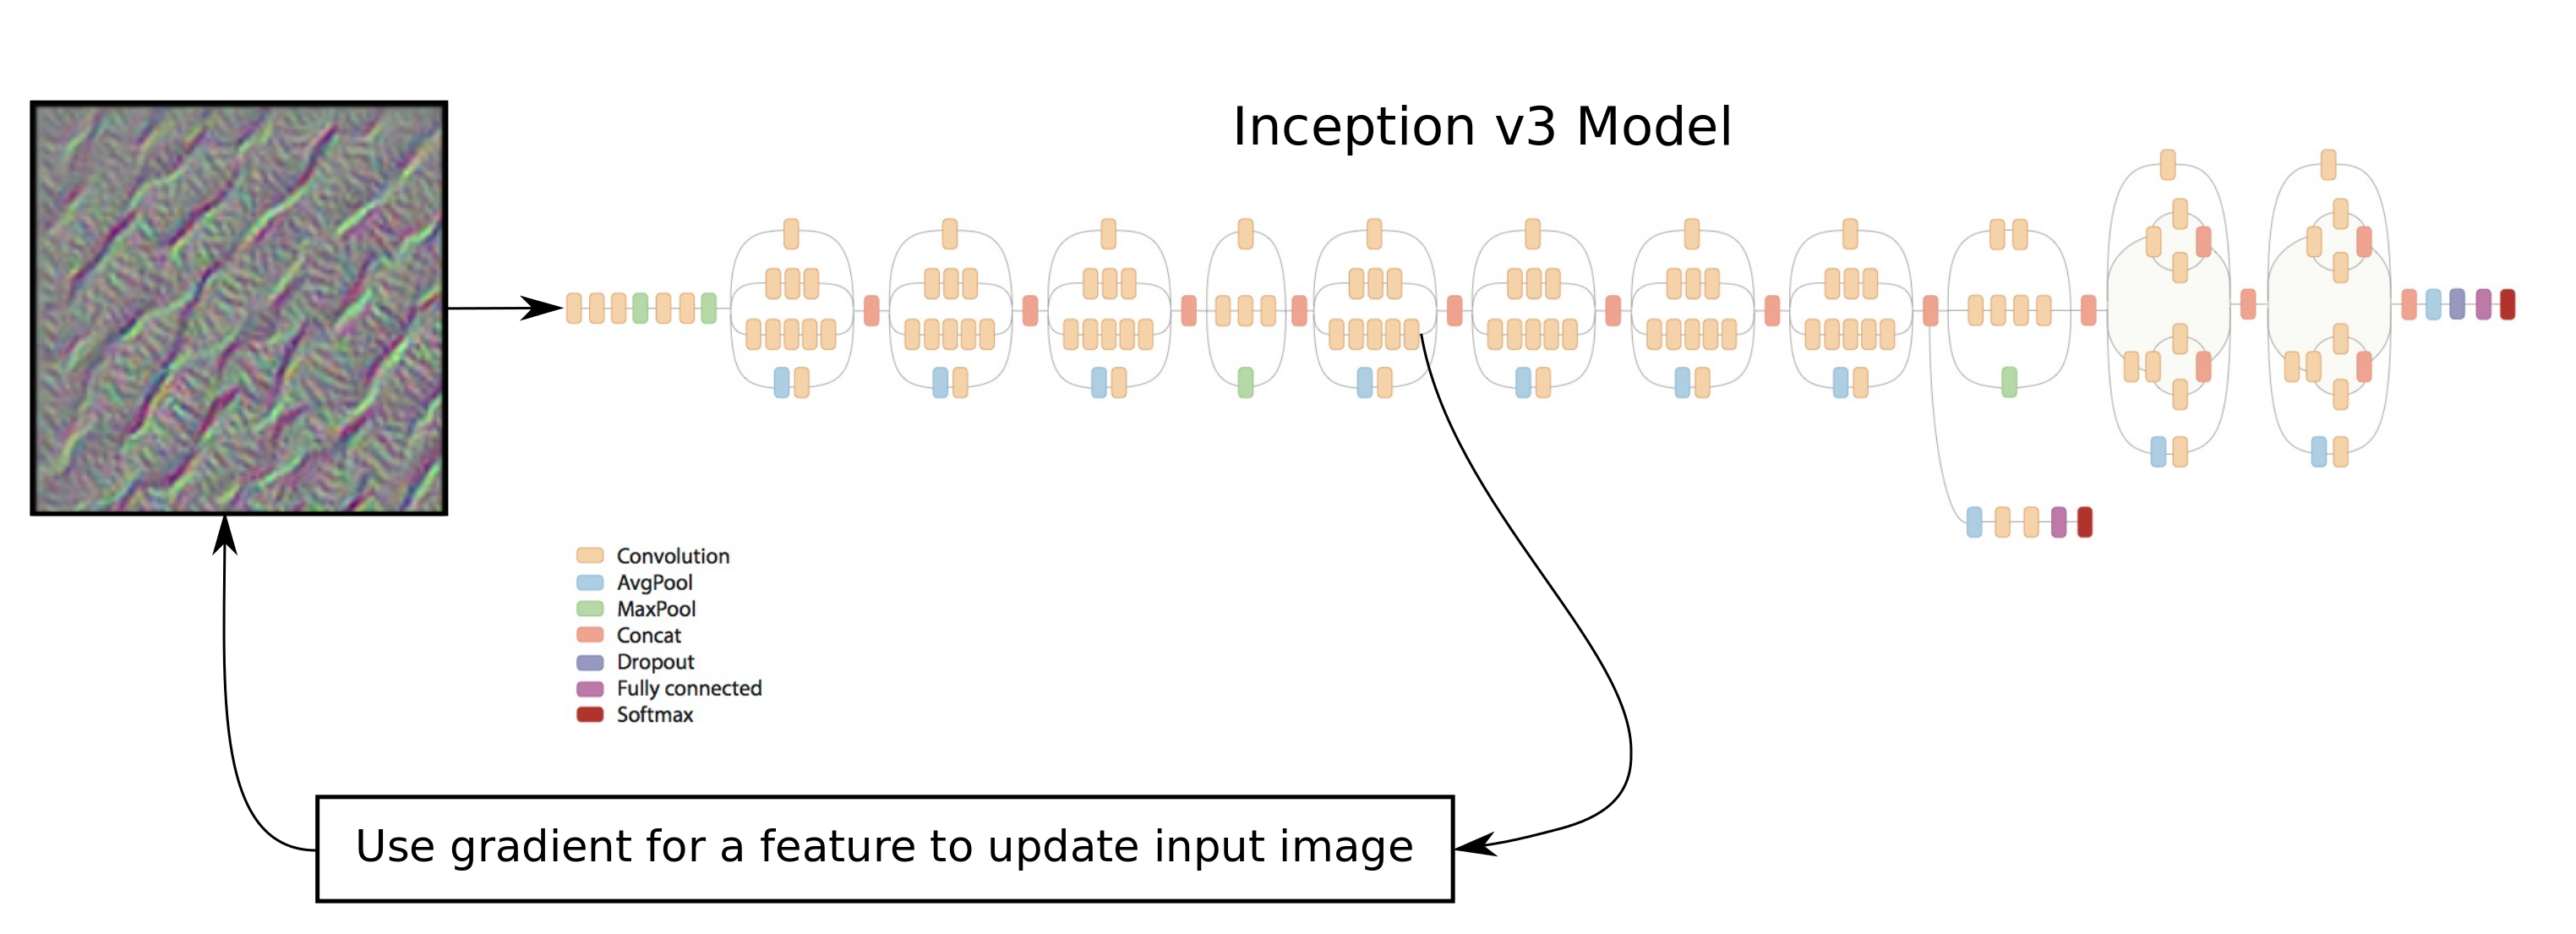
\includegraphics[width=.95\linewidth]{how_nn_see.png}
%\end{center}
%\end{frame}
%
%
%\begin{frame}{Пример из вашей домашки}
%\begin{center}
%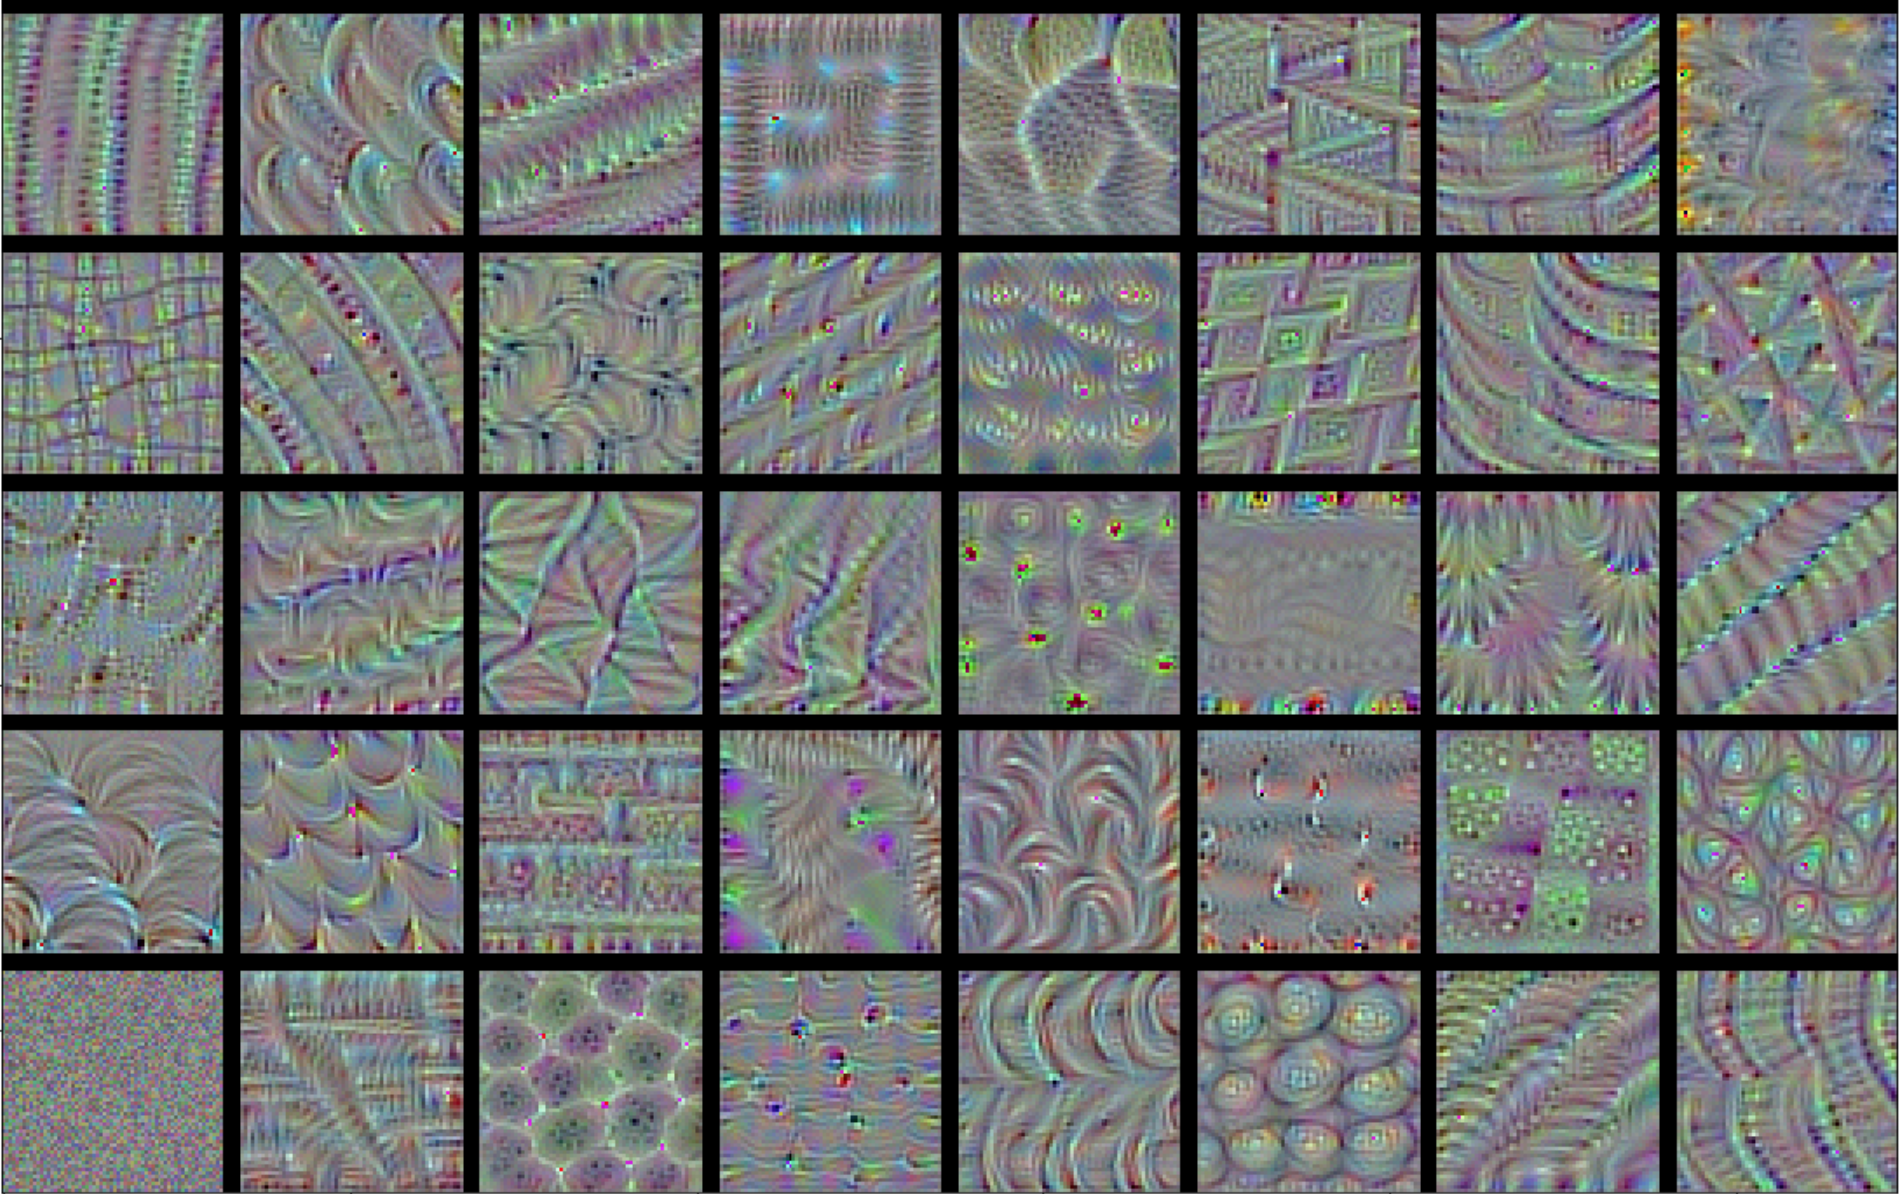
\includegraphics[width=.8\linewidth]{hw_example.png}
%\end{center}
%\end{frame}
%
%\begin{frame}{Что видит свёртка}
%\begin{wideitemize}
%
%\item На вход идет пустое изображение, мы хотим изменить его пиксели так, чтобы активация конкретной свёртки была максимальной 
%
%\item Максимизируем среднее значение свёртки по пикселям 
%
%\item Шаг градиентного спуска: меняем пиксили так, чтобы свёртка выдавала на выход более большие значение 
%
%\item На входной карточке постепенно прорисовывается шаблон, который возбуждает соотвествующую свёртку
%
%\item Если на вход в сетку подсунуть не пустую карточку, а какое-то изображение, то фильтр отрисуется на нём. Если эту процедуру немного подправить, получится наркомания под названием \alert{Deep dream}
%\end{wideitemize}
%\end{frame}
%
%\begin{frame}{Deep dream}
%\begin{center}
%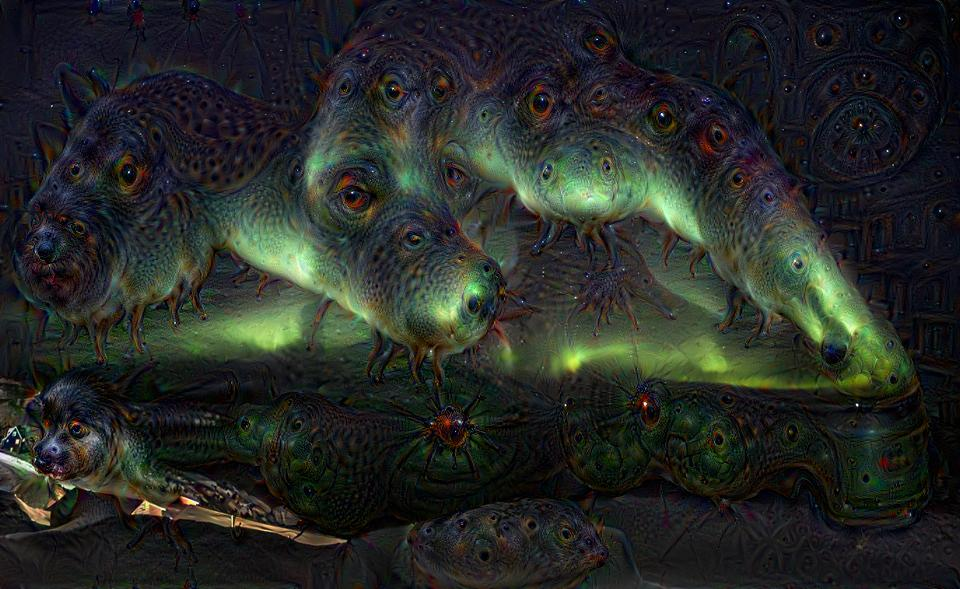
\includegraphics[width=.7\linewidth]{wtf1.jpg}
%\end{center}
%\vfill
%\footnotesize
%{\color{blue} \url{https://nplus1.ru/material/2015/07/13/use}}
%\end{frame}
%
%
%\begin{frame}{Content loss}
%\begin{center}
%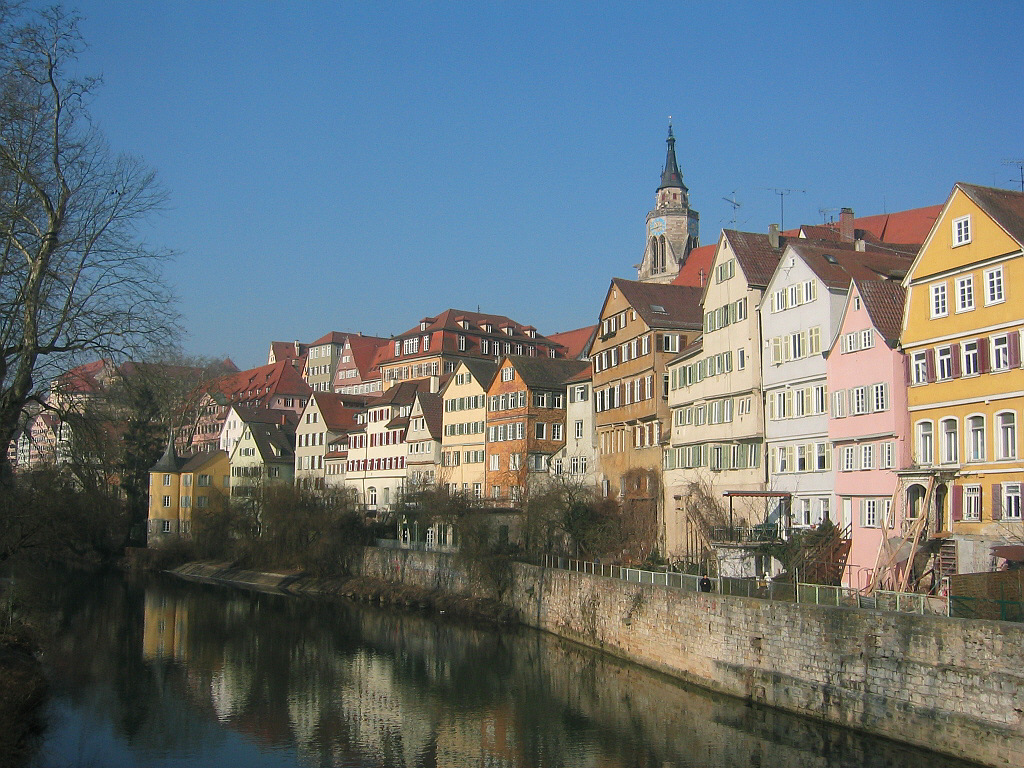
\includegraphics[width=.6\linewidth]{content_image.jpg}
%\end{center}
%\vfill
%\footnotesize
%{\color{blue} \url{https://habr.com/ru/company/mailru/blog/306916/}}
%\end{frame}
%
%\begin{frame}{Content loss}
%\begin{center}
%\includegraphics[width=.5\linewidth]{content1.png}
%\end{center}
%\vfill
%\footnotesize
%{\color{blue} \url{https://habr.com/ru/company/mailru/blog/306916/}}
%\end{frame}
%
%
%
%\begin{frame}{Style loss}
%\begin{center}
%\includegraphics[width=.6\linewidth]{style_image.jpg}
%\end{center}
%\vfill
%\footnotesize
%{\color{blue} \url{https://habr.com/ru/company/mailru/blog/306916/}}
%\end{frame}
%
%\begin{frame}{Style loss}
%\begin{center}
%\includegraphics[width=.5\linewidth]{style1.png}
%\end{center}
%\vfill
%\footnotesize
%{\color{blue} \url{https://habr.com/ru/company/mailru/blog/306916/}}
%\end{frame}
%
%
%\begin{frame}{Смесь нескольких стилей}
%\begin{center}
%\includegraphics[width=.6\linewidth]{brad.png}
%\end{center}
%\vfill
%\footnotesize
%{\color{blue} \url{https://arxiv.org/pdf/1610.07629.pdf}} \ 
%\end{frame}
%
%\begin{transitionframe}
%\begin{center}
%\Huge Переносим стиль!
%\end{center}
%\end{transitionframe}

\end{document}

